\documentclass{statsmsc}

\title{Learning to Bid above a Threshold using Multi-Armed Bandits}
\author{Quentin Leconte}
\CID{2344391}
\supervisor{Ciara Pike-Burke}
\date{31 August 2024}
%For today's date, use:
%\date{\today}
\logoimg{}

% THIS IS WHERE NEW COMMANDS CAN BE DEFINED

% commands below only used in the proof; otherwise can be deleted
\newcommand{\consta}{a}
\newcommand{\X}{X}
\newcommand{\EE}[1]{ \mathrm{E} [ #1 ] }
\newcommand{\inparenth}[1]{\left( #1 \right)}
\usepackage{amsmath}
\usepackage{xcolor}
\usepackage{hyperref}
\usepackage{algorithm}
\usepackage{algpseudocode}
\hypersetup{
    colorlinks,
    linkcolor={blue!50!black},
    citecolor={blue!50!black},
    urlcolor={blue!50!black}
}


\begin{document}

% Generates the Title Page
\maketitle

% Generates plagiarism declaration
\declarationname{Quentin Leconte}
\declarationdate{31 August 2024}
\declaration 

\begin{acknowledgements}

    I would like to thank my supervisor, Professor Ciara Pike-Burke, for her valuable advice and suggestions throughout my research work. I also thank Joseph Lazzaro for his paper recommendations, which were very helpful to me.
\end{acknowledgements}

%=================================================================
% VERY IMPORTANT
% This command switches from Roman to Arabic numbering for main part of report. Do not modify.
\mainmatter
%=================================================================


\begin{abstract}
    This thesis contains my investigations and methods for learning to bid above a threshold. The distribution of the thresholds is considered unknown, and after each bid, only binary feedback is available, indicating whether the bid is above the threshold or not. The objective of this research is 
    to efficiently find, as bids are made, a range of bids that achieves a good tradeoff between the number of bids above the threshold and the bid values, which should not be too high. The methods presented in this thesis are derived from the multi-armed bandit problem (\cite{slivkins2024introductionmultiarmedbandits}).
    Classical methods of the MAB problem are compared to a method specially designed for this study, inspired by Algorithm 1 from the paper \cite{pmlr-v139-cheshire21a}. This thesis seeks an optimal way to approach, with a predetermined precision, a range of bids that maximises the algorithm's total reward. The desired precisions will be associated with a confidence level established using Hoeffding's or Bernstein's inequality.
\end{abstract}

%===============================================================
%
% Students please remove the General tips when submitting your report
%
%===============================================================
% \paragraph{General tips.} Your research report will be judged on the quality of the work it describes according to the Marking Criteria shared with you. 
% When writing your research report you may assume that the reader is familiar with the four core modules of the MSc in statistics. Any additional other material should be explained to the reader, providing suitable references. See Section~\ref{sec:referencing} for more details. For example, you should avoid writing up in detail statistical methods discussed in one of the four core modules, but instead you should briefly present such methods and add appropriate references. More advanced methods or methods discussed in one of the elective modules should be described in more detail and referenced appropriately. 

% Your report must be presented within this template and be at most 35 pages in length, as counted by the Arabic page numerals (1,2,3…). This limit includes all figures and tables presented in the main text, as well as the Endmatter and References sections. This is approximately equivalent to a limit of 15,000 words. Shorter submissions may be graded highly, while excess length disproportionate to the content may be penalised.


% Before submitting the research project, make sure you read the report in its entirety. There should be no half-finished sentences. All mathematical symbols should be defined. Use a spell-checker.

% You will have to submit your report electronically in PDF format through the virtual learning environment (Blackboard). Please name this file in the following format: “CID-Surname-Firstname-Report.pdf”. Your report will be checked for plagiarism via online plagiarism detection services (e.g. Turnitin). 

% Note the report submission deadline is a very hard deadline since the assessment process has then to be completed on a very short timescale.

\section{Introduction}

% \paragraph{Tips for the Introduction.} This is where you describe the topic and the research objectives of your project. 

% You should attempt to set your work in the context of other work previously done in the field. Convey the background of your research referencing earlier work as appropriate. Define core terms. Include background and context, and focus as appropriate on the wider statistical context. Aim to demonstrate that you can confidently describe your project within a broader context of statistical research, as well as scientific research, that goes well beyond the more narrow topic of your project.


% The introduction needs to demonstrate that you are aware of what you are doing, and how it relates to other work that should be properly referenced. 

% Clearly point out your main contributions at the end of the introduction, and provide an overview how the rest of your report is structured and links together. 

% Aim for approximately 1.5-3 pages, similar in style to a general science or statistics research paper.\footnote{Tip: If you choose to use footnotes, do so sparingly.}.


% "
% We consider two different stopping conditions of the game, which are known as fixed confidence
% setting and fixed budget setting in the literature.
% "

The problem studied in this thesis can be illustrated by a concrete situation. Let us suppose that a bidder participates in an auction. In each round of the auction, a product is offered, and only one bid can be made. If this bid is above a threshold, the product is won; otherwise, it is withdrawn. 
The challenge for the bidder is that the distribution of the thresholds is unknown; only the bid value and the information that it is above the threshold are known. However, the threshold values are assumed to be independently and identically distributed. The bidder's goal is to find an optimal 
strategy to win as many products as possible while limiting the value of their bids.

This problem can be associated with the multi-armed bandit (MAB) problem, which is widely described in \cite{slivkins2024introductionmultiarmedbandits}.
The MAB problem consists of several rounds, in which a decision must be made to play one arm from a set of arms (the term "arm" comes from the analogy of the arm of a slot machine that would be played in each round). Each arm corresponds to a random variable with an unknown distribution. 
In each round, the reward is sampled from the distribution of the arm played. The goal of the problem is to find a tradeoff between exploiting the arms that seem to provide the highest rewards and exploring the arms that have been played less to estimate their average reward and potentially discover better arms.


Research involving the MAB problem in the case of a reward depending on a threshold can be found. \cite{NIPS2016_0bf727e9}  studies a set of arms with a threshold for each round for a binary reward, which is the indicator of the sample generated by the arm being above the threshold. A concrete example explained in this paper (p. 2) is the choice of a transportation method to deliver a package with a delivery deadline.
The paper \cite{badanidiyuru2021learningbidcontextualprice} is set in the context of an auction where, in each round, a context is provided to all bidders. The goal is to learn to estimate the value of the product based on the context, as well as to understand the strategies of the other bidders.

In this thesis, the main approach consists of partitioning the space of possible bids into sub-intervals of varying sizes, depending on the desired precision. An arm is associated with each interval. Playing an arm thus involves generating a sample from the uniform distribution over the interval associated with the arm.
In the context of the auction, the lower the values in an interval, the more money the bidder saves. However, since the bidder only wins the product if the threshold is exceeded, low values present the risk of winning nothing.


By partitioning the space of bids, it will be shown that the exploration phase can be optimised to select the arms that maximise the reward. 
In the paper \cite{pmlr-v139-cheshire21a}, a set of arms is assumed to be ordered by their average reward in ascending order. Methods then seek to find two arms whose expectations bracket a threshold value known in advance by halving the exploration zone. As the algorithm progresses, the selected arms become increasingly closer (according to the initially established order) until two final arms are selected. Similarly, the method 
presented in this thesis involves bracketing the arm that maximises the reward during the exploration phase by selecting arms that are progressively closer to the optimal arm, according to the natural order of the intervals in the partition.

The complexity of the problem depends on the initially established partition. Indeed, the smaller the intervals, the more centered the bids of an arm will be. Depending on the variance of the threshold distribution, two closely spaced arms (according to the partition order) will have similar expectations, and they will need to be played a certain number of times to determine which of the two has a better reward with a given level of confidence.


Two approaches can then be explored:
\begin{itemize}
    \item The first involves setting a desired precision in advance, i.e., fixing the partition of the bid space. It is assumed that there is no budget limit; the budget is the total number of rounds. The objective is then to select the best arm with an initially desired confidence level.
    \item The second approach involves setting the budget in advance. The goal of the algorithm is then to update the partition of the bid space as rounds progress, in order to obtain increasingly precise bids by reducing the size of the intervals with each update of the partition. The initial partition has large intervals, and it is updated when an arm is considered the best with a given confidence level.
\end{itemize}

The confidence levels mentioned earlier are calculated using inequalities used in the MAB problem, such as the Hoeffding's inequality or Bernstein's inequality.

The results of the methods in this thesis are compared with the $\epsilon$-Greedy algorithm (\cite{Sutton1998}), in which an exploitation / exploration ratio dependent on the round number is decided in advance. In each round, the exploration phase is chosen with a probability equal to the ratio; otherwise, it is an exploitation phase. They are also compared with the Upper Confidence Bounds (UCB) algorithm that seeks the arm with the highest upper bound of the confidence interval for its expected reward.

\section{Methods}\label{sec:methods}

In this section, an analysis of the problem is conducted to lead to the selection of the methods studied in this thesis.

\subsection{Notations and assumptions}\label{subsec:notation_assumptions}

Notations are introduced and will be used throughout this thesis. Additionally, assumptions are made to specify the problem.

\begin{itemize}
    \item The budget $T$ is the number of rounds, it can be infinite;
    \item Thresholds $\tau_t$ statisfy: for each $t = 1, \dots T$, $\tau_t = \tau + \epsilon_t$, where $\tau$ is a constant
  and $(\epsilon_t)_{t = 1}^T$ i.i.d with mean $0$ and variance $\sigma^2$. For the remainder of this thesis, it is assumed that the threshold distribution follows a normal distribution $\mathcal{N}(\tau, \sigma^2)$;
    \item It is assumed that the thresholds are positive and do not exceed a predetermined finite value $b_{\sup}$ with probabitily close to 1: $\forall t = 1, \dots T \quad \mathbb{P}\left[\tau_t > 0 \right] \approx 1$ and $\forall t = 1, \dots T \quad \mathbb{P}\left[\tau_t < b_{\sup} \right] \approx 1$; $b_{\sup} = 1$ in the simulations.
    \item At each round $t$, a bid $b_t \in \left[0, b_{\sup}\right]$ is made;
    \item At each round $t$, the available information is: $\mathcal{I}_t = \mathbb{I}_{\left\{\tau_t \leq b_t\right\}}$, it is the indicator that the bid is above the threshold.
  \end{itemize}

  Figure \ref{fig:bid-above-threshold}  illustrates, for $t = 1,\dots 20$, the bids that are accepted (i.e., $b_t > \tau_t$) and those that are rejected.


\begin{figure}[htbp]
    \centering
    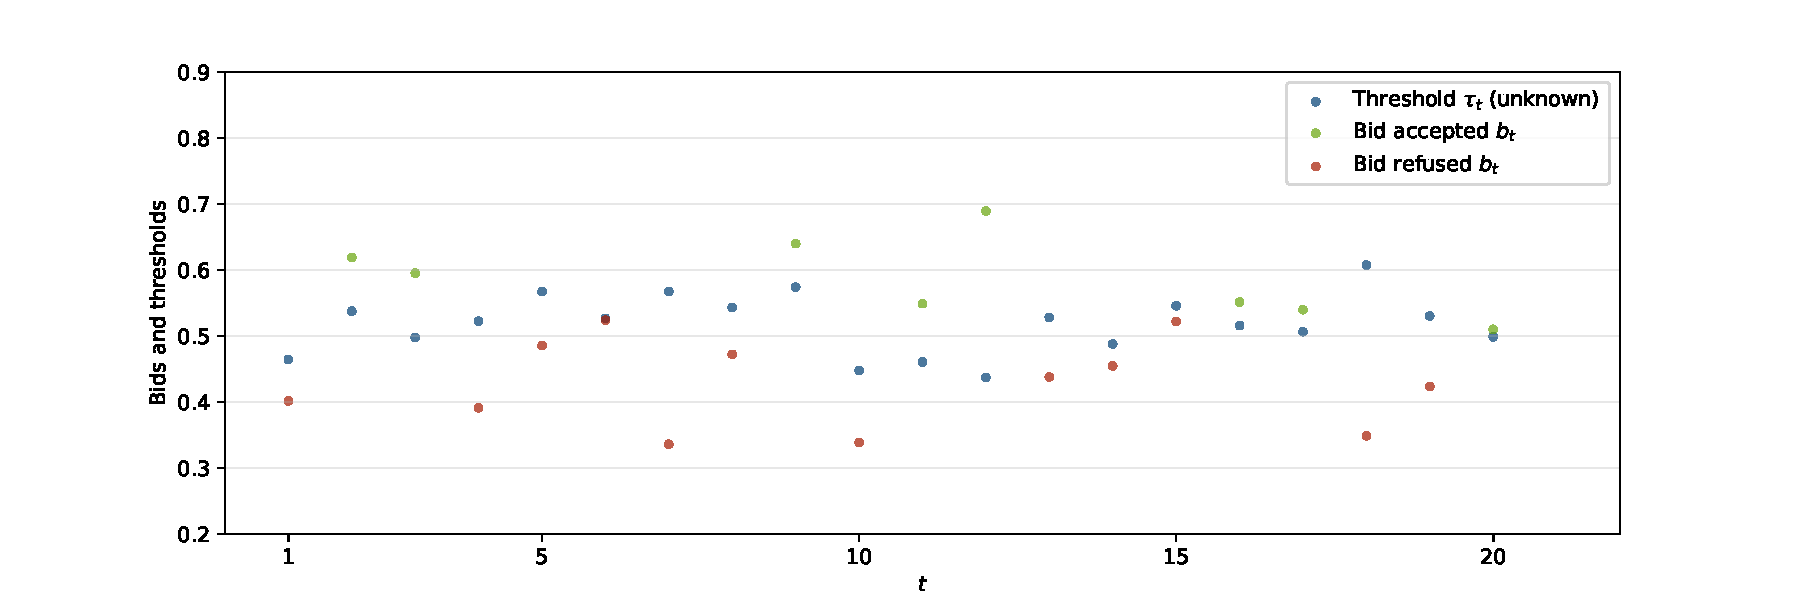
\includegraphics[width=\textwidth]{images/bid_threshold.pdf}
    \caption{Illustration of attempts to bid above a threshold (in blue) over 20 rounds. Bids above the threshold are shown in green, and bids below the threshold are shown in red.}
    \label{fig:bid-above-threshold}
\end{figure}

\subsection{Partition of the bid space and reward function}\label{subsec:reward_partition}

\subsubsection{Partition}
The bid space is partitioned, and an arm is associated with each interval of the partition. 
The bid values range between $0$ and $b_{\sup}$. Assuming that $J$ arms are considered in total, for $j = 1, \dots J$, playing arm $j$ corresponds to making a bid uniformly within the interval:
\[\left[(j-1)\frac{b_{\sup}}{J} , j \frac{b_{\sup}}{J}\right].\]

Increasing the total number of arms $J$ reduces the size of the intervals, leading to arms making more precise bids. Thus, the number 
$J$ controls the precision of the arm considered optimal. For the following, the arm played at round $t$ is denoted by $J_t$.

\subsubsection{Reward and expected reward} 
In round $t$, the reward associated with arm $J_t=j$ that generated the bid $b_t^{(j)}$ is:

\begin{equation}
    X_t^{(j)} = \mathcal{I}_t^{(j)} \left( b_{\sup} - b_t^{(j)}\right)
    \label{eq:reward}
\end{equation}
where $\mathcal{I}_t^{(j)} = \mathbb{I}_{\left\{\tau_t < b_t^{(j)}\right\}}.$

A reward defined as (\ref{eq:reward}) allows for valuing the arms that make low bids as long as they remain above the threshold for the considered round.

It is then possible to calculate the expected reward $\mu_j$ of an arm $j$ associated with a given interval $\left[a_0, a_1 \right]$ ($0\leq a_0 < a_1 \leq b_{\sup})$ by knowing the parameters of the threshold distribution $(\tau, \sigma)$:

\begin{equation}
\begin{aligned}
    \mu_j = &\frac{\sigma}{2(a_1 - a_0)}\biggl( \Phi\left(\tilde{a}_1\right) \left( \sigma - \tilde{a}_1\left(\tau - 2 b_{\sup} + a_1 \right)\right) - \Phi\left(\tilde{a}_0\right) \left( \sigma - \tilde{a}_0 \left(\tau - 2 b_{\sup} + a_0 \right)\right)\\
          &+ \phi\left(\tilde{a}_1\right)\left(  2 ( b_{\sup} - \tau)-\sigma \tilde{a}_1\right) - \phi\left(\tilde{a}_0\right)\left(  2 ( b_{\sup} - \tau)- \sigma \tilde{a}_0\right)\biggr)
  \end{aligned}
  \label{eq:expected_reward}
\end{equation}
  where $\phi$ and $\Phi$ are the PDF and CDF of the standard normal distribution respectively and for $i \in \{0,1\}, \quad \tilde{a}_i = \frac{a_i - \tau}{\sigma}$.

\begin{proof} The threshold distribution $(\tau_t)_t$ is $\mathcal{N}(\tau, \sigma^2)$ and $b_t^{(j)}$ is uniformly distributed in $\left[ a_0, a_1\right]$.
    The PDF and CDF of the standard normal distribution are denoted by $\phi$ and $\Phi$ respectively:
\begin{align*}
    \mu_j &= \mathbb{E}[X_t^{(j)}] \\
    & = \int_{-\infty}^{\infty}\int_{-\infty}^{\infty} \mathbb{I}_{\{x \leq b\}}(b_{\sup}-b) \frac{\phi(\frac{x - \tau}{\sigma})}{\sigma}\frac{\mathbb{I}_{\{a_0 \leq b \leq a_1\}}}{a_1 - a_0} dx db \\
  & = \frac{1}{a_1 - a_0}\int_{a_0}^{a_1}\int_{-\infty}^{b} (b_{\sup}-b) \frac{\phi\left(\frac{x - \tau}{\sigma}\right)}{\sigma} dx db \\
  & = \frac{1}{a_1 - a_0}\int_{a_0}^{a_1} (b_{\sup}-b) \int_{-\infty}^{b} \frac{\phi\left(\frac{x - \tau}{\sigma}\right)}{\sigma} dx db \\
  & = \left[- \frac{(b_{\sup}-b)^2}{2 (a_1 - a_0)} \Phi\left(\frac{b - \tau}{\sigma}\right) \right]_{a_0}^{a_1} + \frac{1}{a_1 - a_0}\int_{a_0}^{a_1}  \frac{(b_{\sup}-b)^2}{2 \sigma} \phi\left(\frac{b - \tau}{\sigma}\right)db.
\end{align*}
And (with $\tilde{a}_0 = \frac{a_{0} - \tau}{\sigma} $ and $\tilde{a}_1 = \frac{a_{1} - \tau}{\sigma}$):
\begin{align*}
  \int_{a_0}^{a_1}  \frac{(b_{\sup}-b)^2}{2 \sigma} \phi\left(\frac{b - \tau}{\sigma}\right)db & = \int_{\tilde{a}_0}^{\tilde{a}_1}  \frac{(b_{\sup}- \sigma b - \tau)^2}{2} \phi\left(b\right)db \\
  & = \frac{1}{2}\left(\sigma^2\int_{\tilde{a}_0}^{\tilde{a}_1} b^2 \phi\left(b\right)db\right. \\
  & + 2 \sigma (\tau - b_{\sup})\int_{\tilde{a}_0}^{\tilde{a}_1} b \phi\left(b\right)db \\
  & + \left.(\tau - b_{\sup})^2 \int_{\tilde{a}_0}^{\tilde{a}_1} \phi\left(b\right)db \right).
\end{align*}

By integration by parts:
\begin{align*}
  &\sigma^2 \int_{\tilde{a}_0}^{\tilde{a}_1} b^2 \phi(b)db = \sigma^2 \left( \Phi\left(\tilde{a}_1\right) -  \Phi\left(\tilde{a}_0\right) - \tilde{a}_1 \phi\left(\tilde{a}_1\right) + \tilde{a}_0 \phi\left(\tilde{a}_0\right)\right)\\
  &2 \sigma (\tau - b_{\sup}) \int_{\tilde{a}_0}^{\tilde{a}_1} b \phi(b)db = 2 \sigma (b_{\sup} - \tau) \left( \phi\left(\tilde{a}_1\right) - \phi\left(\tilde{a}_0\right)\right)\\
  &(\tau - b_{\sup})^2 \int_{\tilde{a}_0}^{\tilde{a}_1} \phi(b)db = (\tau - b_{\sup})^2 \left(\Phi\left(\tilde{a}_1\right) - \Phi\left(\tilde{a}_0\right) \right).
\end{align*}

Finally:
\begin{align*}
  \mu_j = &\frac{\sigma}{2(a_1 - a_0)}\biggl( \Phi\left(\tilde{a}_1\right) \left( \sigma - \tilde{a}_1\left(\tau - 2 b_{\sup} + a_1 \right)\right) - \Phi\left(\tilde{a}_0\right) \left( \sigma - \tilde{a}_0 \left(\tau - 2 b_{\sup} + a_0 \right)\right)\\
        &+ \phi\left(\tilde{a}_1\right)\left(  2 ( b_{\sup} - \tau)-\sigma \tilde{a}_1\right) - \phi\left(\tilde{a}_0\right)\left(  2 ( b_{\sup} - \tau)- \sigma \tilde{a}_0\right)\biggr)
\end{align*}
\end{proof}


Figure \ref{fig:exp-rew} shows the expected rewards for a partition of 50 arms and for different values of the standard deviation of the threshold distribution. 
The different expected reward values are consistent. Indeed, when the arms make bids well above the mean of the threshold distribution, the expected rewards decrease linearly, as the term $(b_t^{j} - b_{\sup})$ in reward expression (\ref{eq:expected_reward}) predominates.
When the arms make bids well below the mean of the threshold distribution, the reward is often 0.
Finally, when they make bids close to the mean value, the effect of $\sigma$ becomes apparent. A large $\sigma$ flattens the peak of the highest expected rewards, while a smaller $\sigma$ allows for better distinction of the arm with the highest expected reward.
\begin{figure}[htbp]
    \centering
    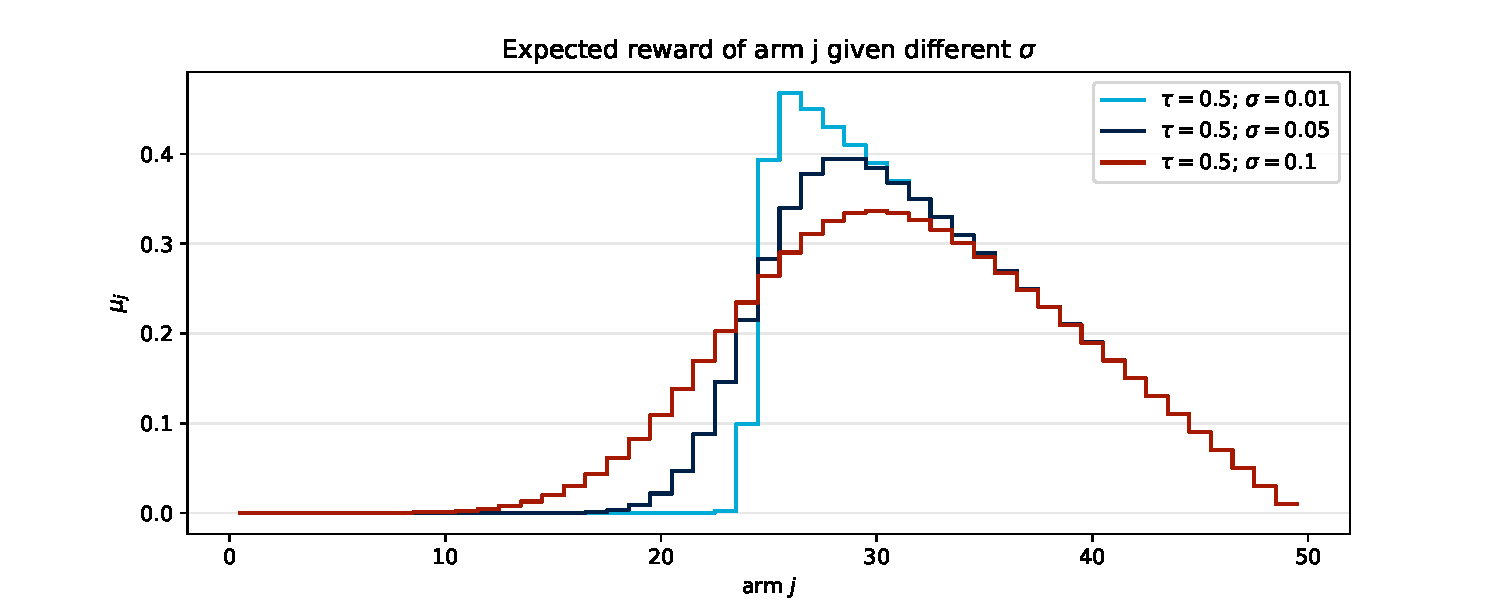
\includegraphics[width=\textwidth]{images/expect_rew_partition50.pdf}
    \caption{Step graph of the expected rewards for each arm for a partition of 50 arms in total. Three configurations are displayed: threshold distribution with a standard deviation $\sigma \in \{0.01, 0.05, 0.1\}$. Moreover, $\tau = 0.5$ and $b_{\sup} = 1$}
    \label{fig:exp-rew}
\end{figure}

In the context of the MAB problem, the expected reward of an arm is not directly accessible. An empirical average reward for each arm $j$ can be constructed using the rewards previously obtained by arm $j$:

\begin{equation}
\hat{\mu}_t^{(j)} = \frac{1}{N_t^{(j)}}\sum_{s=1}^{t} X_{j,s} \mathbb{I}_{\{J_s = j\}}
\label{eq:empirical_exp_rew}
\end{equation}
where $N_t^{(j)}$ is the number of times arm $j$ has been played up to (and including) round $t$.

\subsubsection{Regret of an algorithm}

The regret of an algorithm $\pi$ is a measure of performance in the context of the MAB problem. In round $t$, the regret is updated and corresponds to the sum of the absolute differences between the mean of the optimal arm and the means of the arms chosen in previous rounds $\{J_1, \dots, J_t\}$:

\begin{equation}
    \mathfrak{R}_t(\pi) = \sum_{s=1}^{t}(\mu^* - \mu_{J_t}) 
    \label{eq:regret}
\end{equation}
where $\mu^*$ is the expected reward of the optimal arm. 

Plotting the regret of an algorithm initially allows verifying its convergence towards an optimal arm. Additionally, it enables comparing the efficiency of the exploration phases for the different tested algorithms.

\subsection{Hoeffding and Bernstein inequalities}

In the MAB problem, it is important to estimate the confidence level at which the empirical average reward is a good estimator of the expected reward. It is then beneficial to have a reward distribution that is $\rho$-sub-Gaussian. A variable is $\rho$-sub-Gaussian if its tails fit under a Gaussian distribution.
More precisely, a random variable $X$ is $\rho$-sub-Gaussian with mean $\mu$ if it satisfies the following condition:

\[
\mathbb{E}[e^{\lambda (X - \mu)}] \leq e^{\frac{\lambda^2 \rho^2}{2}}, \quad \text{for all } \lambda \in \mathbb{R}.
\]
\subsubsection{Hoeffding's Inequality}
\begin{lemma}[Hoeffding's Lemma]
  If a random variable takes its values in the interval $[a, b]$ (with $a < b$ and $a,b \in \mathbb{R}$), then it is $\frac{b-a}{2}$-sub-Gaussian.
\end{lemma}

Since the reward distributions (\ref{eq:reward}) take their values in $[0,b_{\sup}]$, it is $\frac{b_{\sup}}{2}$-sub-Gaussian. More precisely, for $j = 1, \dots J$, the reward distribution of arm $j$ takes its values in $\left[0, b_{\sup}\left(1 - \frac{j-1}{J}\right)\right]$, it is thus $b_{\sup}\left(1 - \frac{j-1}{J}\right)/2$-sub-Gaussian.
\begin{theorem}[Hoeffding's Inequality (\cite{Hoeffding1963})]
  Let $X_1, \dots X_N$ be i.i.d. sampled from a $\rho$-sub-Gaussian distribution with expected value $\mu$. Let $\hat{\mu} = \frac{1}{N}\sum_{t = 1}^N X_t$, then for any $\alpha > 0$:
  \begin{equation}
    \mathbb{P}\left[\left|\hat{\mu} - \mu\right|\geq \alpha\right]\leq 2 \exp\left(-\frac{N \alpha^2}{2\rho^2}\right)
    \label{eq:hoeffding}
  \end{equation}  
\end{theorem}

Using (\ref{eq:hoeffding}), for all arm $j$ and for $t = 1, \dots T$, it is possible to bound $\left|\hat{\mu}_t^{(j)} - \mu_j\right|$ with probability greater than $1- \delta$, where $0 <\delta<1$:
 \begin{equation}
  \left|\hat{\mu}_t^{(j)} - \mu_j\right| \leq b_{\sup}\left(1 - \frac{j-1}{J}\right)\sqrt{\frac{\log(2/\delta)}{2 N_t^{(j)}}}
  \label{eq:hoeffding_bound}
\end{equation}
where $N_t^{(j)}$ is suppose to be at least $1$: arm $j$ has been played at least once.

\subsubsection{Bernstein's Inequality}
It is sometimes preferable to use Bernstein's inequality, which involves the variance of the reward distribution.
Indeed, the variance of the reward distribution can be much smaller than the interval in which the reward distribution takes its values. In this case, it is possible to obtain a better bound than Hoeffding's inequality (\ref{eq:hoeffding}).

\cite{foucart13} shows in section 7.5 (Corollary 7.31., p. 179) the Bernstein inequality for bounded random variables.

\usequote{Let $X_1, \dots , X_N$ be independent random variables with zero mean such that $|X_t| \leq K$ almost surely, for $t \in \{1, \dots, N\}$ and some constant $K > 0$. Further assume $\mathbb{E}\left[X_t^2\right] \leq \sigma_t$ for constants $\sigma_t > 0, t \in \{1, \dots N\}$. Then, for
all $\alpha > 0$,
\begin{equation}
\mathbb{P}\left( \left| \sum_{t = 1}^N X_t\right|\geq \alpha\right) \leq 2 \exp\left(-\frac{\alpha^2/2}{\sum_{t = 1}^N \sigma_t^2+K\alpha/3}\right)
\label{eq:bernstein_coro}
\end{equation}
}\citep{foucart13}\footnote{Some notations have been modified to remain consistent with the notations used in the thesis}.

Now, let  $X_1, \dots X_N$ be i.i.d. sampled from a bounded distribution in $[0,b_{\sup}]$ with expected value $\mu$ and variance $v$. 
Let $\hat{\mu} = \frac{1}{N}\sum_{t = 1}^N X_t$, then $\hat{\mu} - \mu = \sum_{t=1}^{N}\frac{X_t - \mu}{N}$ and $\frac{X_1 - \mu}{N}, \dots \frac{X_N - \mu}{N}$ are independent random variables with zero mean and variance $v/N^2$ such that $\left|\frac{X_t - \mu}{N}\right|\leq b_{\sup}/N$ almost surely for $t \in \{1, \dots N\}$.
From Bernstein's inequality (\ref{eq:bernstein_coro}):
\begin{equation}
  \mathbb{P}\left[\left|\hat{\mu} - \mu\right|\geq \alpha\right]\leq 2 \exp\left(-\frac{\alpha^2/2}{\frac{v}{N}+ \frac{b_{\sup} \alpha}{3N}}\right) = 2 \exp\left(-\frac{N \alpha^2}{2 \left(v+ b_{\sup} \alpha/3\right)}\right)
  \label{eq:bernstein}
\end{equation}

\paragraph*{Variance} The variance $v_j$ of the reward distribution of an arm $j$ associated with a given interval $\left[a_0, a_1 \right]$ ($0\leq a_0 < a_1 \leq b_{\sup})$ and given the parameters of the threshold distribution $(\tau, \sigma)$ is :

\begin{equation}
\begin{aligned}
  v_j & = \frac{1}{3(a_1 - a_0)}\biggl(\Phi\left(\tilde{a}_1\right) \left( (b_{\sup}- \tau)^3 +3 \sigma^2 (b_{\sup}- \tau) - (b_{\sup}-a_1)^3\right)\\
  & - \Phi\left(\tilde{a}_0\right) \left( (b_{\sup}- \tau)^3 +3 \sigma^2 (b_{\sup}- \tau) - (b_{\sup}-a_0)^3\right) \\
  & + \phi\left(\tilde{a}_1\right)\left( \sigma^3 \left(\tilde{a}_1^2 + 2 \right) + 3 \sigma (b_{\sup}- \tau)^2 - 3 \sigma^2 (b_{\sup}- \tau)\tilde{a}_1  \right) \\
  & - \phi\left(\tilde{a}_0\right)\left( \sigma^3 \left(\tilde{a}_0^2 + 2 \right) + 3 \sigma (b_{\sup}- \tau)^2 - 3 \sigma^2 (b_{\sup}- \tau)\tilde{a}_0  \right) \biggr) \\
  & - \mu_j^2
  \end{aligned}
  \label{eq:variance_reward}
\end{equation}
  where $\phi$ and $\Phi$ are the PDF and CDF of the standard normal distribution respectively and for $i \in \{0,1\}, \quad \tilde{a}_i = \frac{a_i - \tau}{\sigma}$.

\begin{proof} The threshold distribution $(\tau_t)_t$ is $\mathcal{N}(\tau, \sigma^2)$ and $b_t^{(j)}$ is uniformly distributed in $\left[ a_0, a_1\right]$.
  The second moment of the reward distribution can be calulated:

  \begin{align*}
    \mathbb{E}\left[{X_t^{(j)}}^2\right] &= \mathbb{E}[\mathbb{I}_{\{\tau_t \leq b^{(j)}\}}(b_{\sup}-b^{(j)})^2] \\
    & = \frac{1}{a_1 - a_0}\int_{a_0}^{a_1} (b_{\sup}-b)^2 \int_{-\infty}^{b} \frac{\phi\left(\frac{x - \tau}{\sigma}\right)}{\sigma} dx db \\
    & = \left[- \frac{(b_{\sup}-b)^3}{3 (a_1 - a_0)} \Phi\left(\frac{b - \tau}{\sigma}\right) \right]_{a_0}^{a_1} + \frac{1}{a_1 - a_0}\int_{a_0}^{a_1}  \frac{(b_{\sup}-b)^3}{3 \sigma} \phi\left(\frac{b - \tau}{\sigma}\right)db.
  \end{align*}
  
  And (with $\tilde{a}_0 = \frac{a_{0} - \tau}{\sigma} $ and $\tilde{a}_1 = \frac{a_{1} - \tau}{\sigma}$):
  \begin{align*}
    \int_{a_0}^{a_1}  \frac{(b_{\sup}-b)^3}{3 \sigma} \phi\left(\frac{b - \tau}{\sigma}\right)db & = \int_{\tilde{a}_0}^{\tilde{a}_1}  \frac{(b_{\sup}- \sigma b - \tau)^3}{3} \phi\left(b\right)db \\
    & = \frac{1}{3}\left(- \sigma^3\int_{\tilde{a}_0}^{\tilde{a}_1} b^3 \phi\left(b\right)db\right. \\
    & + 3 \sigma^2 (b_{\sup}- \tau)\int_{\tilde{a}_0}^{\tilde{a}_1} b^2 \phi\left(b\right)db \\
    & - 3 \sigma (b_{\sup}- \tau)^2\int_{\tilde{a}_0}^{\tilde{a}_1} b \phi\left(b\right)db \\
    & + \left.(b_{\sup}- \tau)^3 \int_{\tilde{a}_0}^{\tilde{a}_1} \phi\left(b\right)db \right).
  \end{align*}
    Since: $\sigma^3\int_{\tilde{a}_0}^{\tilde{a}_1} b^3 \phi\left(b\right)db = \sigma^3 \left( \tilde{a}_0^2 \phi(\tilde{a}_0) -\tilde{a}_1^2 \phi(\tilde{a}_1) + 2 \int_{\tilde{a}_0}^{\tilde{a}_1} b \phi(b) db\right)$
  \begin{align*}
    \mathbb{E}\left[{X_t^{(j)}}^2\right] &= \frac{1}{3(a_1 - a_0)}\biggl( (b_{\sup}-a_0)^3 \Phi\left(\tilde{a}_0\right) - (b_{\sup}-a_1)^3 \Phi\left(\tilde{a}_1\right)\\
   & + \sigma^3 \left( \tilde{a}_1^2 \phi(\tilde{a}_1) -\tilde{a}_0^2 \phi(\tilde{a}_0) + 2 \left( \phi\left(\tilde{a}_1\right) - \phi\left(\tilde{a}_0\right)\right) \right)\\
   & + 3 \sigma^2 (b_{\sup}- \tau) \left( \Phi\left(\tilde{a}_1\right) -  \Phi\left(\tilde{a}_0\right) - \tilde{a}_1 \phi\left(\tilde{a}_1\right) + \tilde{a}_0 \phi\left(\tilde{a}_0\right)\right)\\
   & + 3 \sigma (b_{\sup}- \tau)^2 \left( \phi\left(\tilde{a}_1\right) - \phi\left(\tilde{a}_0\right)\right)\\
   & +  (b_{\sup}- \tau)^3 \left(\Phi\left(\tilde{a}_1\right) - \Phi\left(\tilde{a}_0\right) \right)\biggr)\\
  \end{align*}
  Equality \ref{eq:variance_reward} is obtained by rearranging the terms and subtracting by $\mu_j^2$.
\end{proof}

The variances of the reward distributions for different partitions and different threshold distribution parameters are shown in Figure \ref{fig:variance-reward}. For certain arms, it seems appropriate to apply Bernstein's inequality because the variance is much smaller than the range within which the reward distribution takes value.
Moreover, depending on the number of arms in the partition and the desired precision, the variance changes and becomes increasingly larger.
A desire to increase precision would increase the variance of the optimal arm and make the problem more complex.
\begin{figure}[htbp]
  \centering
  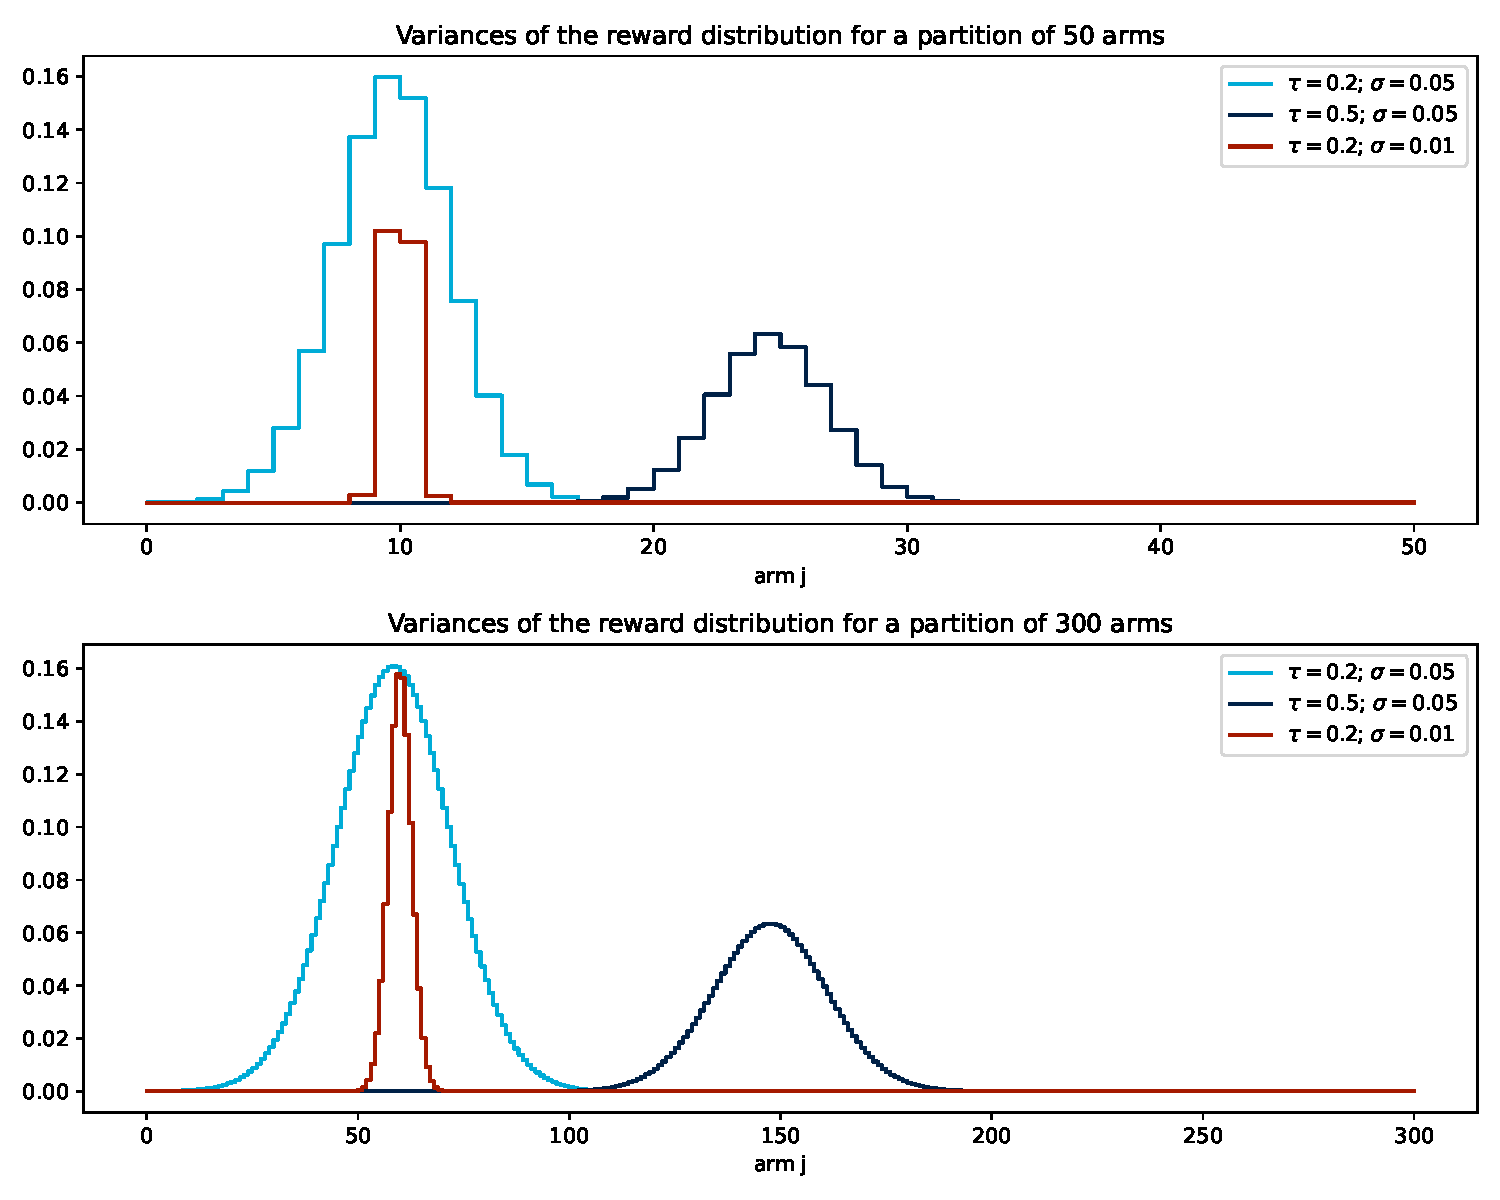
\includegraphics[width=0.7\textwidth]{images/variance_rew_partitions.pdf}
  \caption{Step graph of the variance of the reward distribution for each arm for a partition of 50 and 300 arms. Three configurations are displayed: $\tau = 0.2$ and $\sigma \in \{0.05, 0.01\}$; $\tau = 0.5$ and $\sigma = 0.05$}
  \label{fig:variance-reward}
\end{figure}

Since the variance depends on the unknown parameters of the threshold distribution, it is not possible to use formula (\ref{eq:variance_reward}) to apply Bernstein's inequality (\ref{eq:bernstein_coro}). Instead, for all arm $j$ and for $t = 1, \dots T$, it is possible to use an estimator of the variance:
\[
\hat{v}_t^{(j)} = \frac{1}{N_t^{(j)}}\sum_{s=1}^{t}\left(X_s^{(j)}- \hat{\mu}_t^{(j)}\right)^2 \mathbb{I}_{\left\{J_s = j\right\}}
\]

From the \textit{empirical Bernstein bound} (\cite{mnih:hal-00834983}), with probability at least $1 - \delta$:
\begin{equation}
  \left|\hat{\mu}_t^{(j)} - \mu_j\right| \leq  \sqrt{\hat{v}_t^{(j)}\frac{2\log(3/\delta)}{N_t^{(j)}}} + \frac{3 b_{\sup}\left(1 - \frac{j-1}{J}\right) \log(3/\delta)}{N_t^{(j)}}
  \label{eq:empirical_bernstein}
\end{equation}

Subsequently, the formulas for Hoeffding (\ref{eq:hoeffding_bound}) and Bernstein (\ref{eq:empirical_bernstein}) bounds will provide a confidence level when the algorithms calculate the estimators of the expected rewards of the tested arms.

\subsection{Non-adaptative exploration and exploitation algorithm: epsilon-greedy}

The $\epsilon$-greedy algorithm (\cite{Sutton1998}) serves as a benchmark for testing algorithms specifically designed for this problem. 
After partitioning the bid space into $J$ intervals corresponding to $J$ arms, the first step of the algorithm is to play each arm once for $J$ rounds. The second step, for round $t = J+1, \dots$, involves playing an arm randomly with probability $\epsilon_t > 0$ and playing the arm with the highest empirical average reward (\ref{eq:empirical_exp_rew}) with probability $1 - \epsilon_t$ (see Algorithme \ref{code:epsilon_greedy}).
This algorithm alternates between exploitation and exploration phases to increase the total reward while also discovering better arms.

\begin{algorithm}[H]
    \caption{Epsilon-greedy algorithm}
    \label{code:epsilon_greedy}
    \begin{algorithmic}[0]
    \Require Number of arms $J$ (partition of $[0, b_{\sup}]$), strategy exploration / exploitation $(\epsilon_t)_t^T$
    \For{$ j = 1, \dots, J$} \Comment{Initialisation}
    \State Play arm $j$ bidding uniformly in its interval and get $X_j^{(j)}$
    \State Update $\hat{\mu}^{(j)}_j$
    \EndFor
    \For{$ t = J+1, \dots, T$}
    \If{Uniform$([0,1]) < \epsilon_t$} \Comment{Exploration}
    \State Choose randomly $j^* \in \{1, \dots J\}$
    \Else \Comment{Exploitation}
    \State $j^* = \text{argmax}_{j \in \{1, \dots J\}} (\hat{\mu}^{(j)}_t)$
    \EndIf
    \State Play arm $j^*$ bidding uniformly in its interval and get $X_t^{(j^*)}$.
    \State Update $\hat{\mu}^{(j)}_j$
    \EndFor
  \end{algorithmic}
  \end{algorithm}

It is necessary to find a strategy to parameterise the evolution of the exploration probability $\epsilon_t$ over the rounds. According to Theorem 1.6 (p7) of \cite{slivkins2024introductionmultiarmedbandits}, choosing $\epsilon_t = t^{-1/3} (J \log(t))^{1/3}$ will achieve regret bound $\mathbb{E}\left[\mathfrak{R}_t\right]\leq t^{2/3} O\left(J \log(t)\right)^{1/3}$ for each round $t$. 

This algorithm will prioritise maximising short-term reward through its exploitation phase. However, even though the exploration probability decreases over the rounds, there is no stopping criterion that allows for the selection of an optimal arm at the end of the algorithm; hence, the algorithm is designed to run indefinitely. 
It is indeed not adaptive, because it does not take into account the information obtained about the expected rewards of the played arms to construct confidence intervals.
Studying its regret is still relevant for comparison with algorithms 
that have a stopping criterion but may incur significantly more regret before finding the optimal arm.

\subsection{Optimistic algorithm: Upper Confidence Bound (UCB) algorithm}

The UCB algorithm (\cite{ucbcitation}) plays all the arms and calculates the upper bound of their confidence intervals according to the formulas derived from 
Hoeffding or Bernstein inequalities. The algorithm then decides to play the arm with the highest upper bound at each round. These upper bounds can be large for two reasons: the expected reward is high, or the arm has been played few times. 
Thus, over the rounds, the confidence interval bounds will tighten, allowing the algorithm to exploit arms that have not been played much.

Based on the formulas (\ref{eq:hoeffding_bound}) or (\ref{eq:empirical_bernstein}), the UCB can be calculated with parameter $\delta >0$ and for arm $j = 1, \dots J$ and round $t = 1, \dots T$.

From Hoeffding's inequality:
\begin{equation}
 \text{UCB}^{(j)}_t(\delta) = \hat{\mu}_t^{(j)} + b_{\sup}\left(1 - \frac{j-1}{J}\right)\sqrt{\frac{\log(2/\delta)}{2 N_t^{(j)}}}
 \label{eq:UCB_hoeffding}
\end{equation}
From Bernstein's inequality:
\begin{equation}
  \text{UCB}^{(j)}_t(\delta) = \hat{\mu}_t^{(j)} +\sqrt{\hat{v}_t^{(j)}\frac{2\log(3/\delta)}{N_t^{(j)}}} + \frac{3 b_{\sup}\left(1 - \frac{j-1}{J}\right) \log(3/\delta)}{N_t^{(j)}}.
\label{eq:UCB_bernstein}
\end{equation}

The UCB algorithm for the problem raised in this thesis is presented in Algorithm \ref{code:UCB}.

\begin{algorithm}[H]
  \caption{UCB algorithm}
  \label{code:UCB}
  \begin{algorithmic}[0]
  \Require Number of arms $J$ (partition of $[0, b_{\sup}]$), confidence parameter $\delta>0$
  \For{$ j = 1, \dots, J$} \Comment{Initialisation}
  \State Play arm $j$ bidding uniformly in its interval and get $X_j^{(j)}$
  \State Update $\hat{\mu}^{(j)}_j$, $\text{UCB}^{(j)}_t(\delta)$
  \EndFor
  \For{$ t = J+1, \dots, T$}
  \State $j^* = \text{argmax}_{j \in \{1, \dots J\}} (\text{UCB}^{(j)}_{t-1}(\delta))$
  \State Play arm $j^*$ bidding uniformly in its interval and get $X_t^{(j^*)}$.
  \State Update $\hat{\mu}^{(j)}_j$, $\text{UCB}^{(j)}_t(\delta)$
  \EndFor 
\end{algorithmic}
\end{algorithm}

\subsection{Adaptative sequential halving algorithm}

Observing Figure \ref{fig:exp-rew}, which shows the expected rewards as a function of the arms arranged in the order of the partition intervals, a single local maximum, which is global as well, is observed. Therefore, it is pertinent to create an algorithm that seeks a maximum. The algorithm presented in this section is inspired
by Algorithm 1 of \cite{pmlr-v139-cheshire21a}, which aimed to bracket a threshold value between two arms from a set of arms that were arranged in ascending order of their expected rewards.

The sequential halving algorithm in this thesis operates in episodes of three rounds, during which three arms are played and their empirical average rewards are updated at round $t$. The relative values of the empirical average rewards determine the three arms that will be played in round $t+1$.
The three arms will be denoted by $\{L_t, M_t, R_t\}$ for left, middle, right. There are then three configurations of interest at round $t$:
\begin{itemize}
  \item $\hat{\mu}_t^{(L_t)} \geq \hat{\mu}_t^{(M_t)} \geq \hat{\mu}_t^{(R_t)}$: ascending configuration;
  \item $\hat{\mu}_t^{(L_t)} \leq \hat{\mu}_t^{(M_t)} \leq \hat{\mu}_t^{(R_t)}$: descending configuration;
  \item $\hat{\mu}_t^{(L_t)} < \hat{\mu}_t^{(M_t)}$ and $\hat{\mu}_t^{(R_t)} < \hat{\mu}_t^{(M_t)}$: peak configuration;
  \item otherwise: other configuration. 
\end{itemize}

Each configuration corresponds to a rule for activating the three new arms (see Figure \ref{fig:seq-halving}).
\begin{itemize}
\item Ascending: $L_{t+1} \leftarrow M_t$; $M_{t+1} \leftarrow R_t$; $R_{t+1} \leftarrow 2R_t - M_t$ (right shift).
\item Descending: $L_{t+1} \leftarrow 2L_t - M_t$; $M_{t+1} \leftarrow L_t$; $R_{t+1} \leftarrow M_t$ (left shift).
\item Peak $L_{t+1} \leftarrow \left\lfloor \frac{L_t + M_t}{2} \right\rfloor$; $M_{t+1} \leftarrow M_t$; $R_{t+1} \leftarrow \left\lfloor \frac{R_t + M_t}{2} \right\rfloor$ (halving).
\item Other: keep same arms.
\end{itemize}

\begin{figure}[htbp]
  \centering
  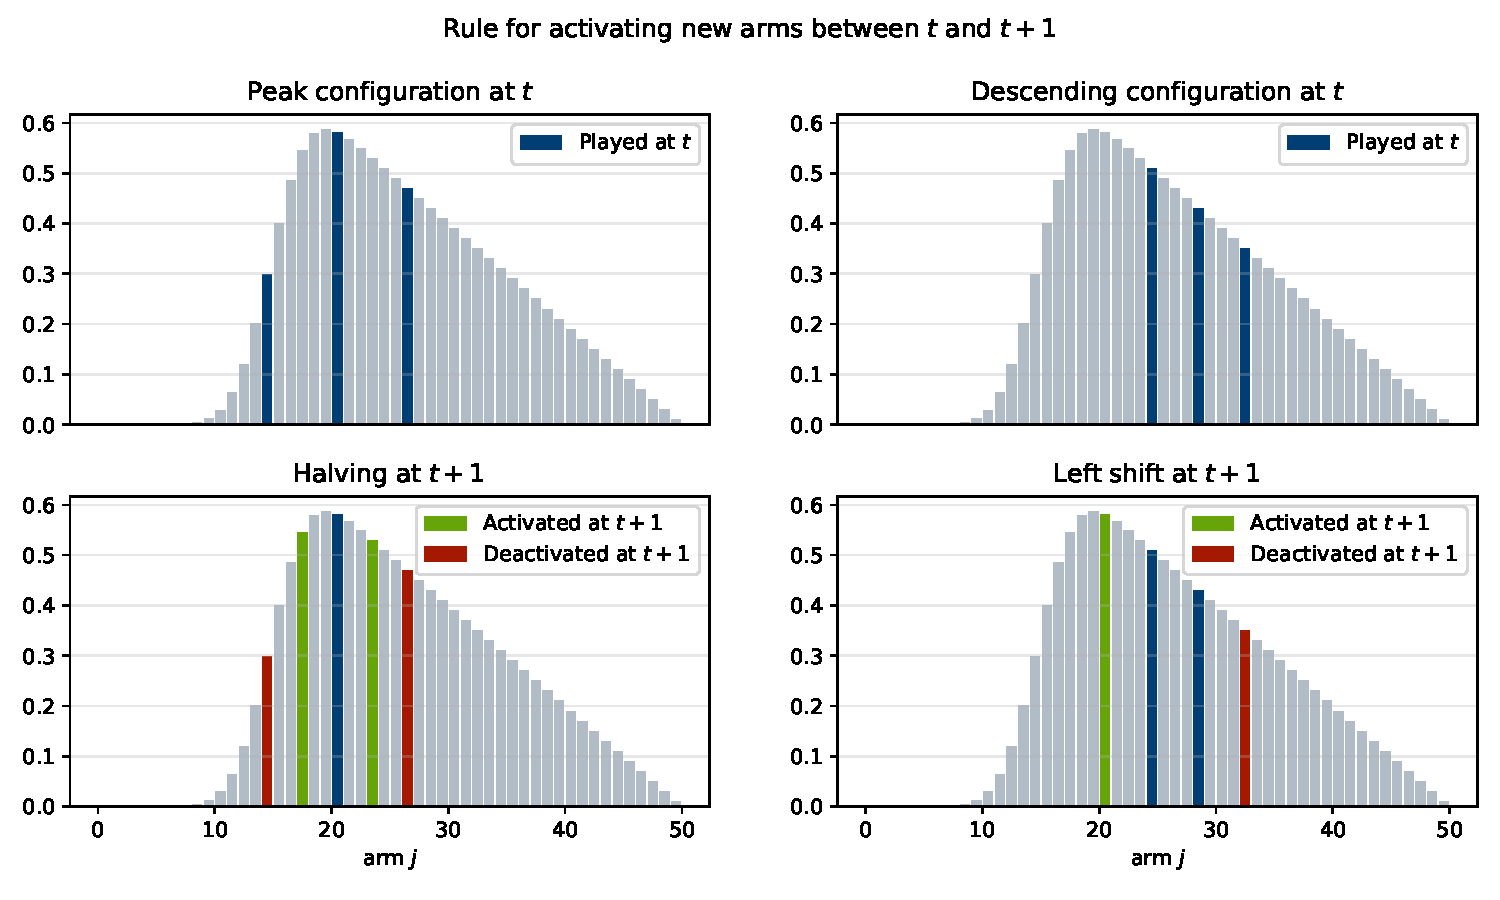
\includegraphics[width=\textwidth]{images/sequential_halving.pdf}
  \caption{Illustration of the choice of new arms to play for the sequential halving algorithm between t and t+1. The left part of the figure shows the case where the three arms seem to surround a peak at round $t$, and the algorithm refines the search by performing a halving at $t+1$. The right part shows the case where the three arms are in a descending configuration at $t$, and the algorithm shifts to the left at $t+1$.}
  \label{fig:seq-halving}
\end{figure}

The case of "other configuration" is possible because the empirical average rewards are not necessarily expected to respect the relative values of the expected rewards. However, this configuration is not stable, and by continuing to play the same arms, one of the three previously described configurations should eventually occur.
It is relevant to note that in the ascending and descending configurations, it is possible for the new arms to be less than $0$ (for $L_{t+1}$) or greater than J (for $R_{t+1}$). In this case, the new arms are 1 (for $L_{t+1}$) or $J$ (for $R_{t+1}$).

This search and halving phase continues until three consecutive arms are obtained. 
Then, the three final arms are played until a confidence interval (based on Hoeffding's or Bernstein's inequality) is built to deduce the optimal arm. The lower confidence bounds (LCB) corresponding to the other inequalities are introduced as well:

From Hoeffding's inequality:

\begin{equation}
  \text{LCB}^{(j)}_t(\delta) = \hat{\mu}_t^{(j)} - b_{\sup}\left(1 - \frac{j-1}{J}\right)\sqrt{\frac{\log(2/\delta)}{2 N_t^{(j)}}}
\label{eq:LCB_hoeffding}
\end{equation}
From Bernstein's inequality:
\begin{equation}
\text{LCB}^{(j)}_t(\delta) = \hat{\mu}_t^{(j)} - \sqrt{\hat{v}_t^{(j)}\frac{2\log(3/\delta)}{N_t^{(j)}}} - \frac{3 b_{\sup}\left(1 - \frac{j-1}{J}\right) \log(3/\delta)}{N_t^{(j)}}.
\label{eq:LCB_bernstein}
\end{equation}

If a peak configuration occurs and the UCB of the left and right arm are lower than the LCB of the middle arm, the algorithm chooses the middle arm as optimal and stops. If an ascending or descending configuration occurs, a shift is performed. The algorithm is described in detail in Algorithm \ref{alg:SHA}.

\begin{algorithm}[H]
  \caption{Adaptative Sequential Halving Algorithm}
  \label{alg:SHA}
    \begin{algorithmic}
      \Require Number of arms $J$ (partition of $[0, b_{\sup}]$), confidence parameter $\delta>0$
      \State \textbf{Initialize:} Episode 0: $L, M, R \gets1,\lfloor J/2 \rfloor,  J$
      \For{Episode $ep = 1, \dots$}
        \State \textbf{Play} arms $L, M, R$ once.
        \State $t_{ep}$ is the final round number of episode $ep$
        \If{$L,M,R$ are consecutive arms}
          \If{$\text{UCB}^{(L)}_{t_{ep}}(\delta)<\text{LCB}^{(M)}_{t_{ep}}(\delta)$ and $\text{UCB}^{(R)}_{t_{ep}}(\delta)<\text{LCB}^{(M)}_{t_{ep}}(\delta)$}
          \State \Return arm M \Comment{The best arm is the current middle arm}
          \EndIf
          \If{$\text{UCB}^{(2)}_{t_{ep}}(\delta)<\text{LCB}^{(1)}_{t_{ep}}(\delta)$}
          \State \Return arm 1 \Comment{The best arm is the one at the far left}
          \EndIf
          \If{$\text{UCB}^{(J-1)}_{t_{ep}}(\delta)<\text{LCB}^{(J)}_{t_{ep}}(\delta)$}
          \State \Return arm J \Comment{The best arm is the one at the far right}
          \EndIf
        \EndIf
        \If{$\hat{\mu}_{t_{ep}}^{L} < \hat{\mu}_{t_{ep}}^{M}$ and $\hat{\mu}_{t_{ep}}^{R}< \hat{\mu}_{t_{ep}}^{M}$} \Comment{Peak configuration}
          \State $L, M, R \gets \lfloor (L + M)/2\rfloor, M, \lfloor (R + M + 1)/2\rfloor$
        \EndIf
        \If{$\hat{\mu}_{t_{ep}}^{L} \leq \hat{\mu}_{t_{ep}}^{M} \leq \hat{\mu}_{t_{ep}}^{R}$} \Comment{Ascending configuration}
          \State $L_{\text{new}}, M_{\text{new}}, R_{\text{new}} \gets \min(M, J-2), \min(R, J-1), \min(2R - M, J)$
        \EndIf
        \If{$\hat{\mu}_{t_{ep}}^{L} > \hat{\mu}_{t_{ep}}^{M} > \hat{\mu}_{t_{ep}}^{R}$} \Comment{Descending configuration}
          \State $L_{\text{new}}, M_{\text{new}}, R_{\text{new}} \gets \max(2 L - M, 1), \max(L, 2), \max(M, 3)$
        \EndIf
        \State $L, M , R \gets L_{\text{new}}, M_{\text{new}}, R_{\text{new}}$
      \EndFor
     \end{algorithmic}

  \end{algorithm}
\section{Results}

This section shows the results of the algorithms presented in Section \ref{sec:methods}. The algorithms are compared in terms of their accuracy, efficiency, and convergence. 
In the first approach, the objective of the algorithms is to find the optimal arm given a specified partition. Their regrets can be studied until the optimal arm is confidently obtained. 
In the second approach, the sequential halving algorithm will be used to find a range of bids given a fixed budget decided in advance. 
The goal of the algorithm will be to refine the partition as the optimal arms are confidently identified.

\subsection{Analysis of the confidence parameter in the case of the Sequential Halving Algorithm}

The Upper Confidence Bounds (\ref{eq:UCB_hoeffding}, \ref{eq:UCB_bernstein}) and Lower Confidence Bounds (\ref{eq:LCB_hoeffding}, \ref{eq:LCB_bernstein}) used in the Sequential Halving Algorithm depend on a confidence parameter. In the code, the UCB and LCB are slightly modified to account for $\delta$ values between 0 and 1.

From Hoeffding's inequality, the tested UCB and LCB for arm $j$ and round $t$ are:
\begin{subequations}\label{eq:hoeffding_test}
  \begin{align}
    \text{UCB}^{(j)}_t(\delta) &= \hat{\mu}_t^{(j)} + b_{\sup}\left(1 - \frac{j-1}{J}\right)\sqrt{\frac{\log(1/\delta)}{2 N_t^{(j)}}} \label{eq:UCB_hoeffding_test} \\ 
    \text{LCB}^{(j)}_t(\delta) &= \hat{\mu}_t^{(j)} - b_{\sup}\left(1 - \frac{j-1}{J}\right)\sqrt{\frac{\log(1/\delta)}{2 N_t^{(j)}}} \label{eq:LCB_hoeffding_test}.
  \end{align}
\end{subequations}
From Bernstein's inequality, the tested UCB and LCB for arm $j$ and round $t$ are:
\begin{subequations}\label{eq:bernstein_test}
  \begin{align}
    \text{UCB}^{(j)}_t(\delta)&=\hat{\mu}_t^{(j)} - \sqrt{\hat{v}_t^{(j)}\frac{2\log(1/\delta)}{N_t^{(j)}}} + \frac{3 b_{\sup}\left(1 - \frac{j-1}{J}\right) \log(1/\delta)}{N_t^{(j)}} \label{eq:UCB_bernstein_test} \\ 
    \text{LCB}^{(j)}_t(\delta)&=\hat{\mu}_t^{(j)} - \sqrt{\hat{v}_t^{(j)}\frac{2\log(1/\delta)}{N_t^{(j)}}} - \frac{3 b_{\sup}\left(1 - \frac{j-1}{J}\right) \log(1/\delta)}{N_t^{(j)}} \label{eq:LCB_bernstein_test}.
  \end{align}
\end{subequations}

\subsubsection{The required number of iterations according to the value of the confidence parameter}

For the simulations, it is necessary to estimate the number of times the last three arms $L$, $M$, and $R$ need to be played to stop Algorithm \ref{alg:SHA}, assuming that arm $M$ is optimal. Knowing the formula for the expected reward (\ref{eq:expected_reward}) given a partition and a threshold distribution, it is possible to calculate the distance between arms $M$ and $L$, 
and between arms $M$ and $R$. With these distances, it is possible to calculate the number of times the arms need to be played so that the LCB of arm $M$ is greater than the UCBs of arms $L$ and $R$, given a value of $\delta \in (0,1)$. For the UCB and LCB calculated using Bernstein's inequality, the formula for the variance of the reward distribution (\ref{eq:variance_reward}) is used.

The distance between the expected reward of arm $j$ and the expected reward of arm $i$ is denoted by $\Delta_{i,j}$. 
Assuming that arm $j$ is the optimal arm, the number of times the arms need to be played given $\delta \in (0,1)$ is (from Hoeffding's inequality):
\begin{equation}
  n_{\text{Hoeffding}}(\delta) \geq \max_{i \in \{j-1, j+1 \}} 2 \log\left(\frac{1}{\delta}\right)\left(\frac{b_{\sup}\left(1 - \frac{(j+i)/2 - 1}{J}\right)}{\Delta_{i,j}}\right)^2
  \label{eq:n_hoeffding}
\end{equation}
Assuming that arm $j$ is the optimal arm, the number of times the arms need to be played given $\delta \in (0,1)$ is (from Bernstein's inequality):
\begin{equation}
  n_{\text{Bernstein}}(\delta) \geq \max_{i \in \{j-1, j+1 \}} 2\log\left(\frac{1}{\delta}\right) \left(\frac{\sigma_{i,j} + \sqrt{\sigma_{i,j}^2 +3 \Delta_{i,j} b_{\sup} (1 -\frac{ (j+i)/2 - 1}{J}) }}{\Delta_{i,j}}\right)^2
  \label{eq:n_bernstein}
\end{equation}
where $\sigma_{i,j} = \frac{\sqrt{v_j} + \sqrt{v_i}}{2}$, for $i \in \{j-1, j+1\}$

Figure \ref{fig:delta_test} shows the evolution of the number of times the three best arms (the optimal arm as the middle arm and the two others left and right) need to be played so that the LCB of the optimal arm is higher than the UCBs of the two other surrounding arms (left and right) given $\delta$ for several partitions with different threshold distributions.

\begin{figure}[htbp]
  \centering
  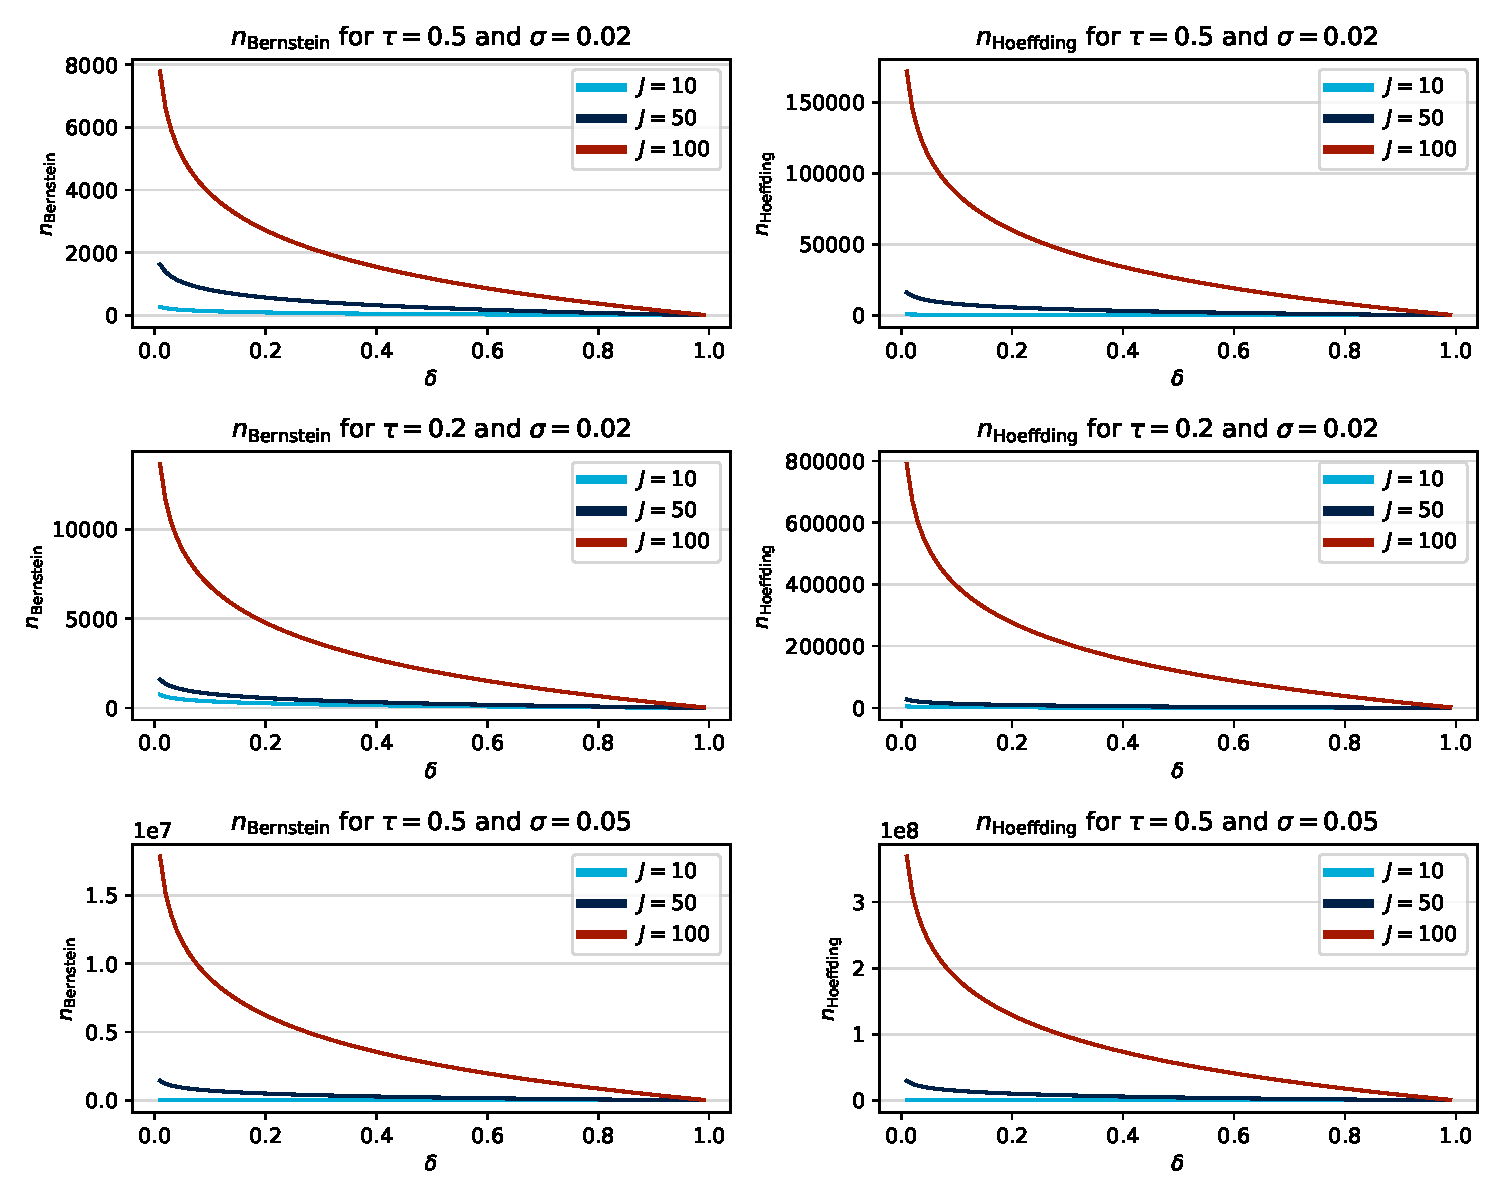
\includegraphics[width=\textwidth]{images/n_bernstein_hoeffding.pdf}
  \caption{Comparison of the number of times the top three arms must be played to select the optimal arm, given the confidence parameter $\delta$. Multiple threshold distributions are tested, and for each, three more or less precise partitions are used. On the left, the confidence parameter uses Bernstein bounds ()\ref{eq:n_bernstein}); on the right, it uses Hoeffding bounds (\ref{eq:n_hoeffding}).}
  \label{fig:delta_test}
\end{figure}


By observing Figure \ref{fig:delta_test}, the bounds constructed using Bernstein's inequality (\ref{eq:UCB_bernstein_test}, \ref{eq:LCB_bernstein_test}) result in a lower number of iterations compared to those constructed with Hoeffding's inequality (\ref{eq:UCB_hoeffding_test}, \ref{eq:LCB_hoeffding_test}) for the same confidence parameter. However, the Bernstein bounds require the calculation of the variance of rewards, which increases the complexity of the computations and, consequently, the computation time

\subsubsection{Success probability of the Sequential Halving Algorithm according to the values of the confidence parameter}

Here, several values of $\delta$ are tested for a given partition and threshold distribution to observe the number of successes of the sequential algorithm, providing an estimate of its success probability for a given $\delta$ value.

Figure \ref{fig:succes_rate} shows the success rates after 5000 simulations of the Sequential Halving algorithm. The partition includes $J = 30$ arms, and the standard deviation of the threshold distribution is set at $\sigma = 0.02$. The means $\tau = 0.3, 0.5, 0.7$ of the threshold distribution are tested for different $\delta$ values.

\begin{figure}[htbp]
  \centering
  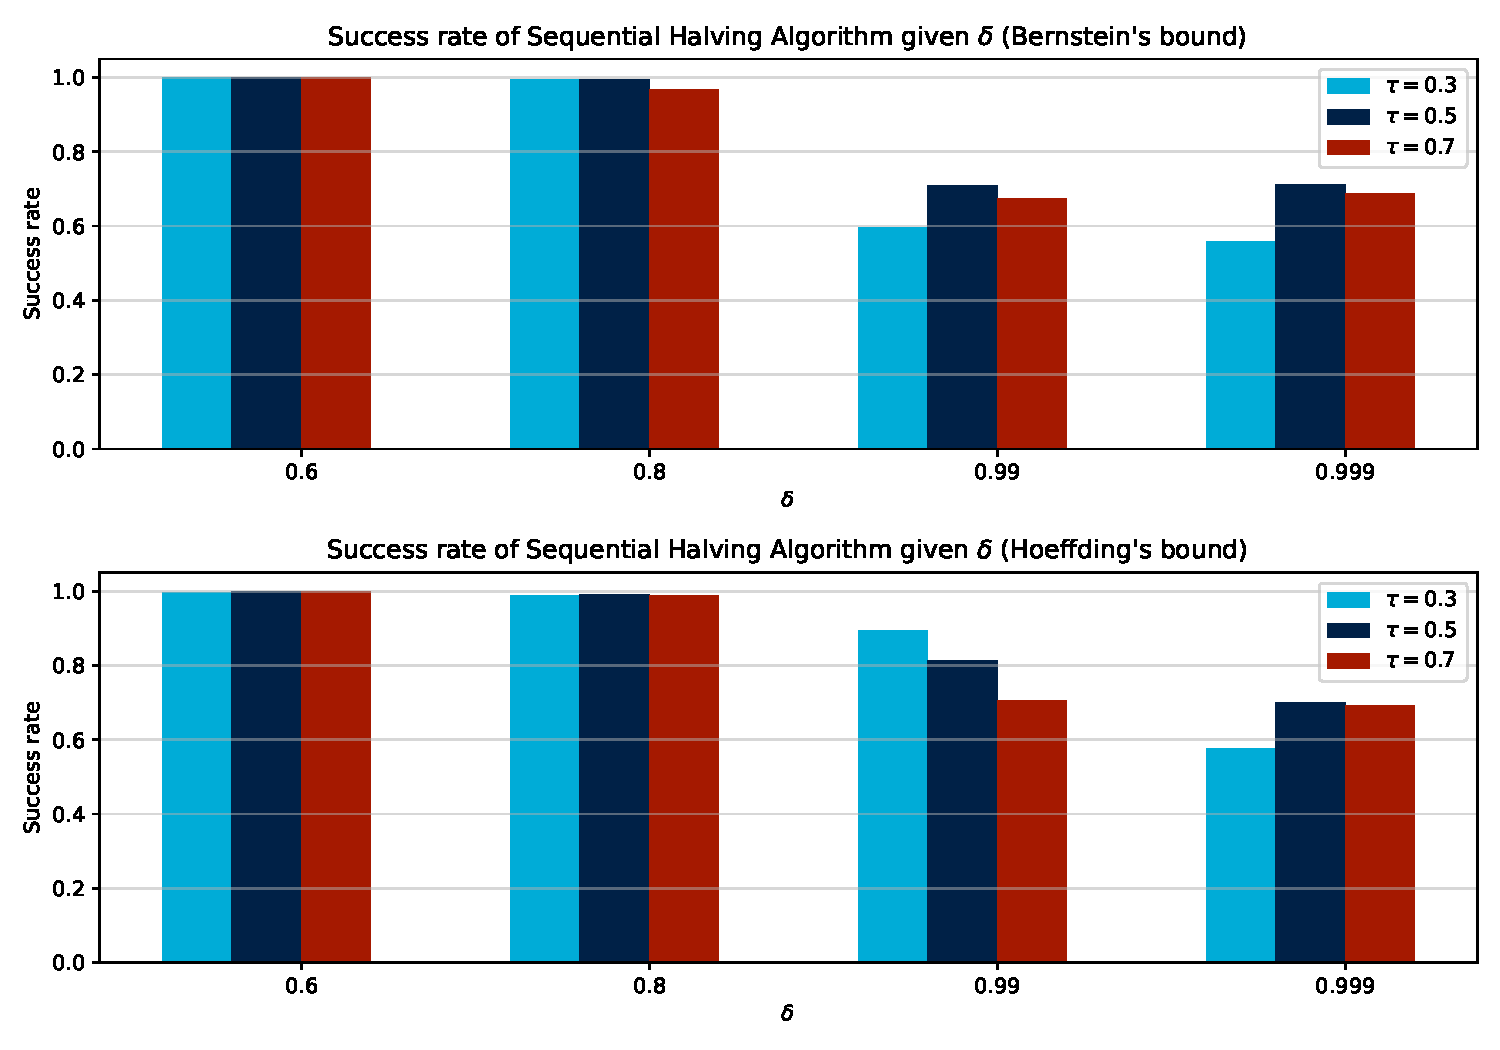
\includegraphics[width= 0.7\textwidth]{images/delta_test.pdf}
  \caption{Bar plot of the success rates of the sequential halving algorithm with Bernstein's and Hoeffding's bounds. The standard deviation of the threshold distribution 
  is $\sigma = 0.02$ and the partition consists of 30 arms. Confidence parameters $\delta \in \{0.6, 0.8, 0.99, 0.999\}$ and threshold distribution means $\tau \in \{0.3, 0.5, 0.7\}$ are tested.}
  \label{fig:succes_rate}
\end{figure}
For both types of bounds, a confidence parameter below $0.8$ will yield a success rate close to 1. In the simulations, a confidence parameter below $0.6$ provides a success rate of 1. Therefore, to avoid excessively long computation times, the confidence parameter will be set at $0.6$ to ensure results with significant confidence.

\subsection{Comparison of the Regret of the Different Tested Algorithms}


The regrets of the $\epsilon$-Greedy (\ref{code:epsilon_greedy}), UCB (\ref{code:UCB}), and Sequential Halving (\ref{alg:SHA}) algorithms are displayed for 50 simulations of three different partitions ($J \in \{10, 50, 100\}$) and for each of the bounds (Bernstein in Figure \ref{fig:regret_bern} and Hoeffding in Figure \ref{fig:regret_hoeff}). The distribution of the thresholds is 
$\mathcal{N}(0.5, 0.02)$ and the budget is $T = 5000$.

\begin{figure}[htbp]
  \centering
  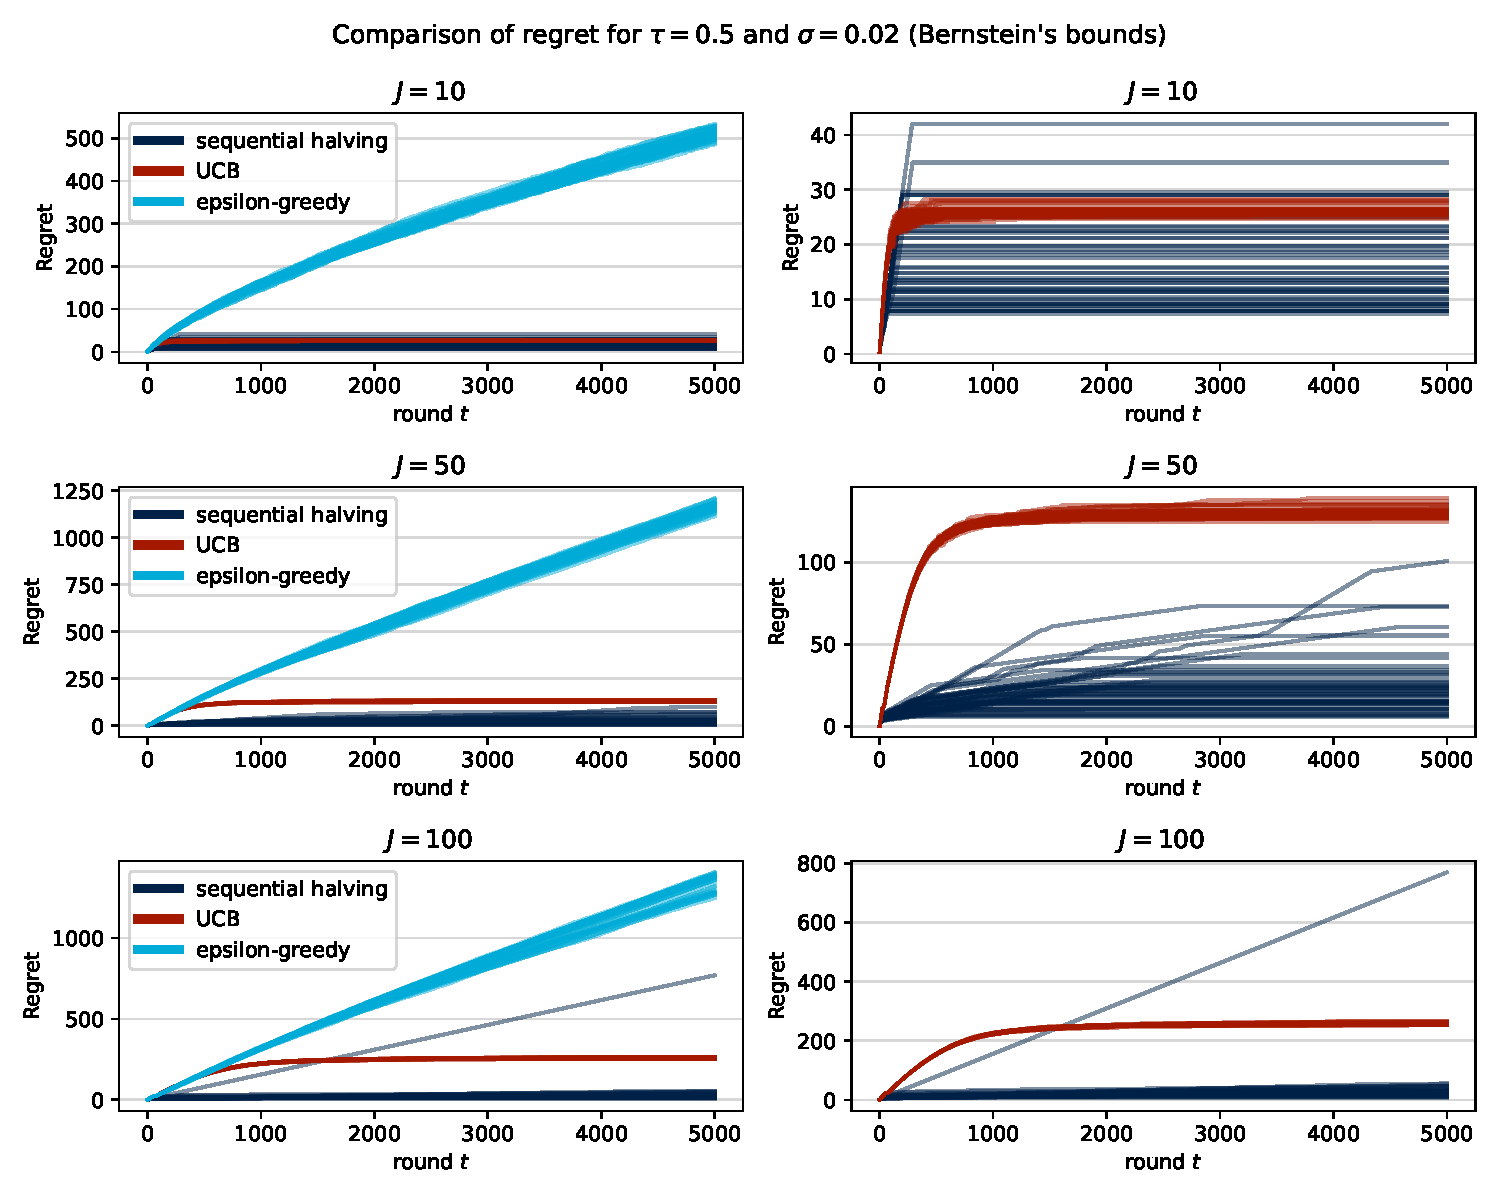
\includegraphics[width=0.8 \textwidth]{images/regret.pdf}
  \caption{Comparison of regret using the Bernstein's bound for $J \in \{10, 50, 100\}$. On the left, the regrets of the three algorithms are displayed; on the right, the same regrets but only for the UCB and Sequential Halving algorithms.}
  \label{fig:regret_bern}
\end{figure}

\begin{figure}[htbp]
  \centering
  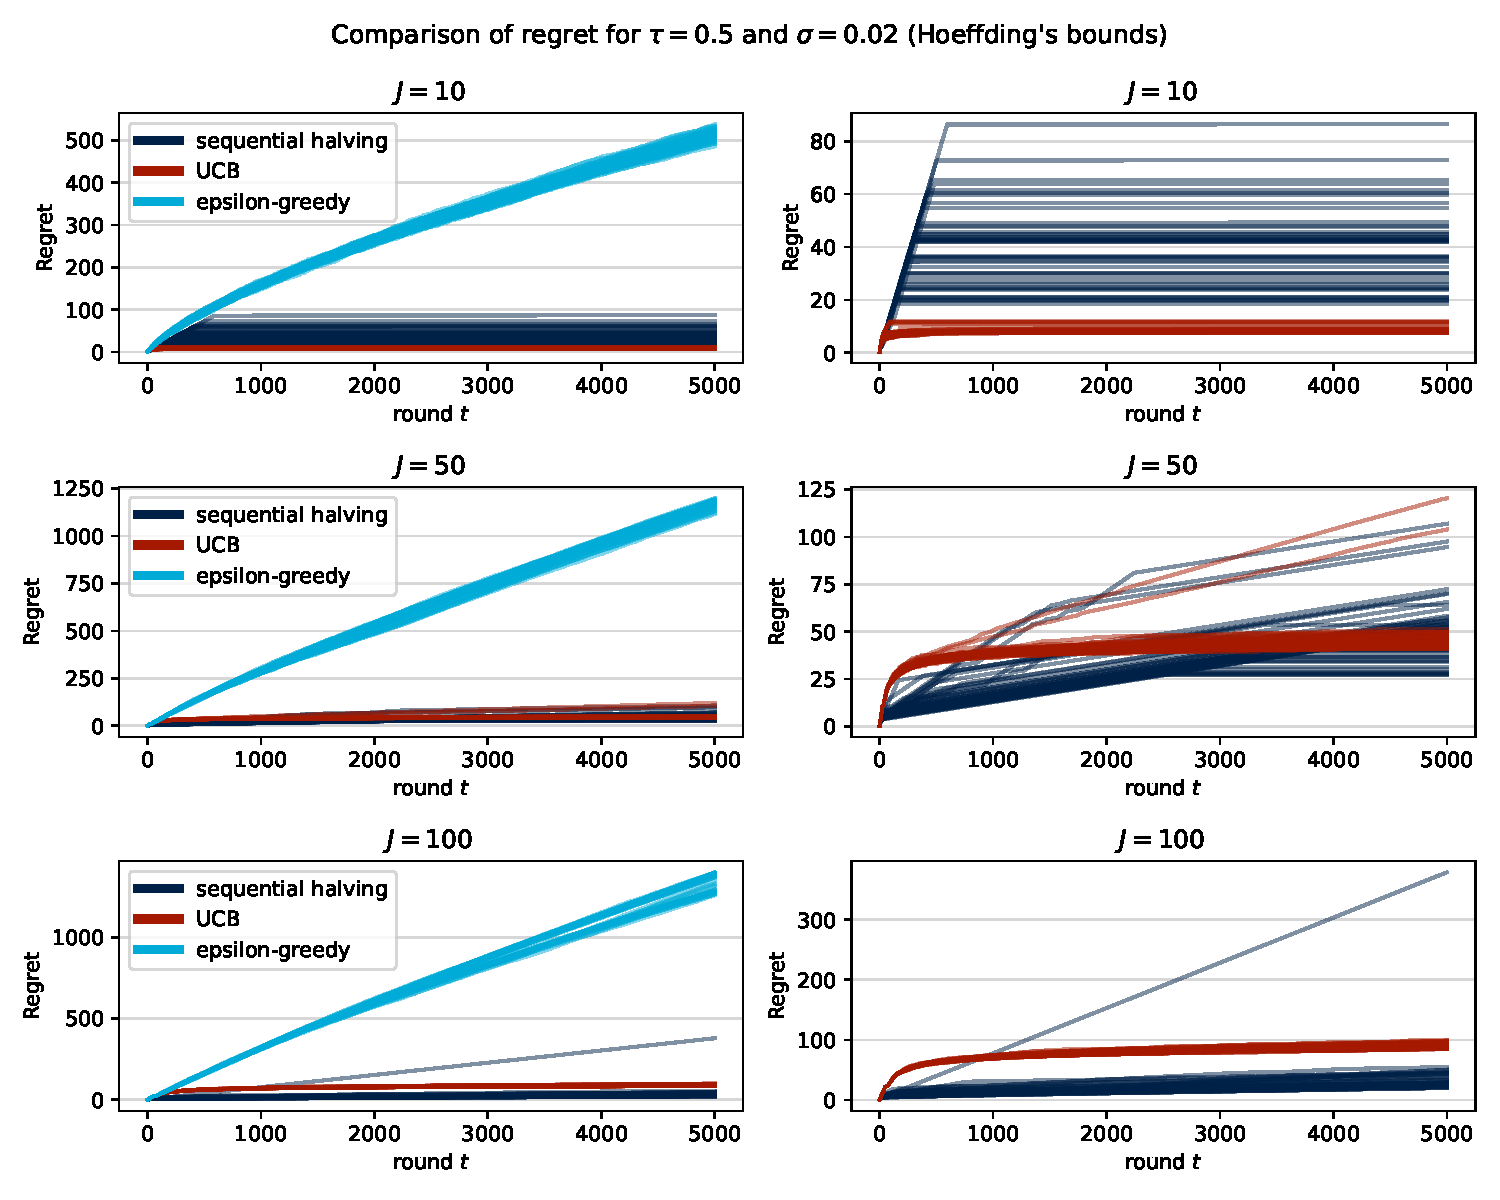
\includegraphics[width=0.8 \textwidth]{images/regret_hoeffding.pdf}
  \caption{Comparison of regret using the Hoeffding's bound for $J \in \{10, 50, 100\}$. On the left, the regrets of the three algorithms are displayed; on the right, the same regrets but only for the UCB and Sequential Halving algorithms.}
  \label{fig:regret_hoeff}
\end{figure}

By observing Figures \ref{fig:regret_bern} and \ref{fig:regret_hoeff}, it is clear that the $\epsilon$-Greedy algorithm underperforms regardless of the configurations. For Bernstein's bound, the Sequential Halving algorithm appears to perform better than UCB, particularly for partitions with a large number of arms (J in 50, 100). Conversely, the UCB algorithm seems to perform better with Hoeffding's bound, especially for partitions with 10 and 50 arms, but not for the partition with 100 arms.

Additionally, it is important to note that with Hoeffding's bound and for partitions with 50 and 100 arms, the Sequential Halving algorithm does not have enough rounds to select the optimal arm, which is why it does not converge. This is not the case for the UCB algorithm, which appears much more stable. Indeed, by design, the UCB algorithm incurs significant regret in the early rounds because it tests all the arms uniformly until it naturally focuses on testing only the optimal one. In contrast, the Sequential Halving algorithm quickly narrows down what it believes to be the top three arms and then tests them sequentially to select the optimal one with the desired confidence level.

\subsection{Using the Sequential Halving algorithm to narrow down the range of optimal bids given a fixed budget}

Here, the second approach to this problem is tested. With a predetermined budget, how can we obtain the smallest possible range of optimal bids with a certain degree of confidence?

Algorithm \ref{alg:ZoomSha} involves repeating the Sequential Halving algorithm while updating the partition, which becomes more refined with each repetition. The algorithm takes as input a budget and a number of arms
$J$ for each partition update. In each iteration of the algorithm, the top three consecutive arms are selected, and their union forms the new interval, which will be partitioned into
$J$ arms for the next iteration.

\begin{algorithm}[H]
  \caption{Zooming Sequential Halving Algorithm}
  \label{alg:ZoomSha}
    \begin{algorithmic}
      \Require Number of arms $J$, confidence parameter $\delta>0$, budget $T$
      \State \textbf{Initialisation} $t = 0$, partition of $J$ arms
      \While{$t < T$}
      \State $L, M, R \gets$ Selected left, middle, right arms of Sequential Halving Algorithm \ref{alg:SHA} on partition 
      \State partition $ = $ Union of the intervals associated with $L, M, R$ divided into $J$ arms
      \State $t = t + $ number of rounds needed for the Sequential Halving Algorithm convergence
      \EndWhile
      \Return Union of the intervals associated with $L, M, R$
     \end{algorithmic}
  \end{algorithm}


An example of interval search using Algorithm \ref{alg:ZoomSha} is presented in Figure \ref{fig:zoom}.

\begin{figure}[htbp]
  \centering
  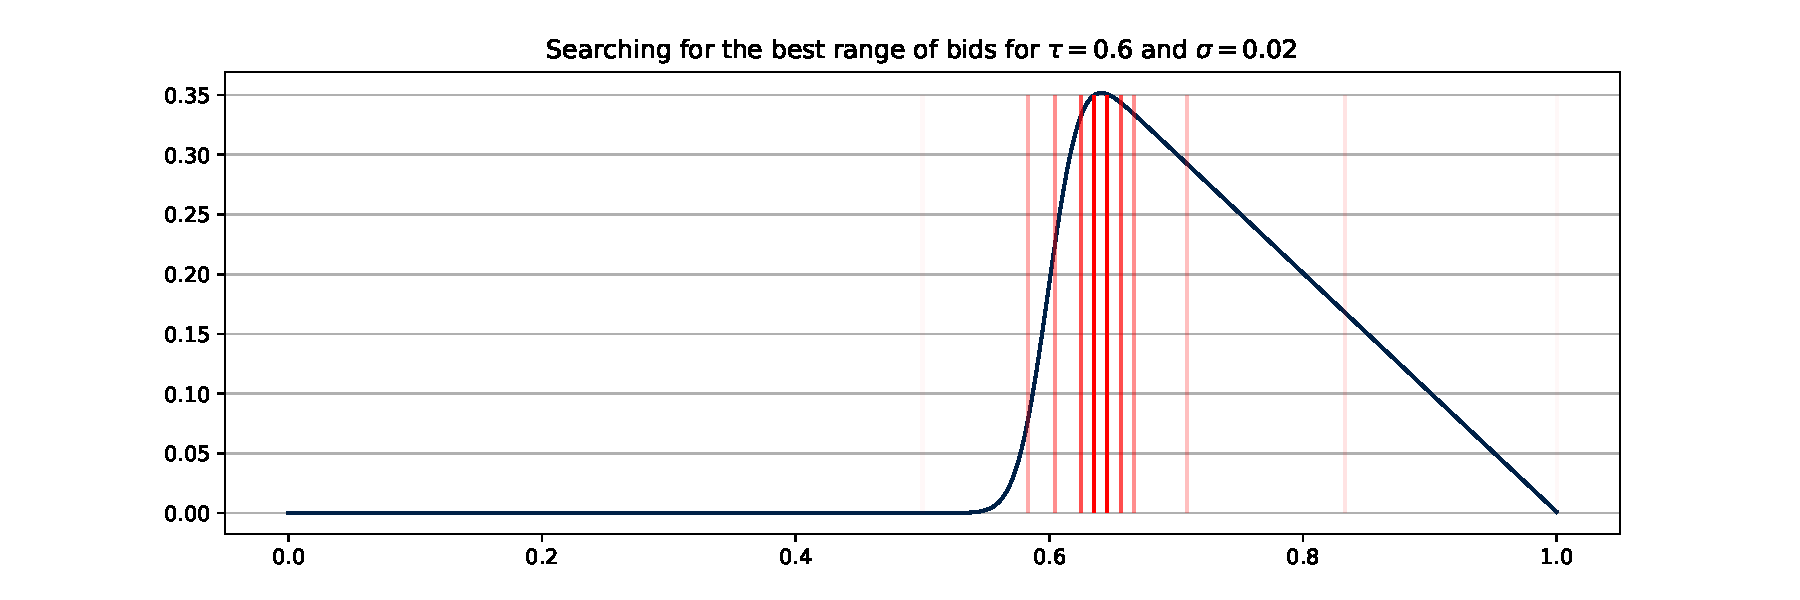
\includegraphics[width=0.8 \textwidth]{images/zooming.pdf}
  \caption{An example of searching for a range of bids with a confidence parameter $\delta = 0.4$, using successive partitions of $J=6$ arms, and with a threshold distribution following $\mathcal{N}(0.6, 0.02)$. The red vertical lines indicate the bounds of the bid intervals chosen progressively by Algorithm \ref{alg:ZoomSha}. The selected interval becomes increasingly precise and is always contained within the previously selected intervals.}
  \label{fig:zoom}
\end{figure}

\section{Discussion}

In this thesis, the multi-armed bandit problem was used to learn how to bid above a threshold. The approach taken in this thesis was to partition the bidding space into intervals where bids are made uniformly. 

The goal of the Sequential Halving algorithm presented was to provide better performance 
than the usual algorithms for the multi-armed bandit problem. The algorithm aimed to efficiently search for the optimal arm within a given partition. The shape of the reward distributions 
for the arms in this problem allowed for the development of a strategy to conduct effective exploration and exploitation phases, enabling confident selection of the optimal arm while minimizing regret. Compared to the UCB algorithm, which appears to converge, the Sequential Halving algorithm outperforms in the case of more precise partitions.


A number of works address the multi-armed bandit problem with reward distributions dependent on a threshold. The paper \cite{pmlr-v139-cheshire21a} is similar to this thesis. In that paper, the goal is to place a threshold between the expected values of the reward distributions of two arms among a set of arms arranged in ascending order of their expectations. Here, the placement of the arms 
is also crucial, as it reveals the existence of a unique maximum. The Sequential Halving algorithm, therefore, seeks to eliminate half of the arms without having to play them each time three arms played appear to surround a maximum.

However, further study is needed on the confidence parameter appearing in Algorithms \ref{code:UCB} and \ref{alg:SHA}. Indeed, the Bernstein's and Hoeffding's inequalities have been used to bound the probability that the arm considered optimal is not actually optimal. But this bound still seems too large compared to the results observed during simulations. 

Finally, the Bernstein's inequality appears more precise than the Hoeffding's inequality, as it helps limit the budget required to select the best arm. However, calculating confidence intervals based on the Bernstein's inequality is more complex and requires longer computation times. Therefore, it is necessary to decide whether the goal is to limit the budget—meaning the total number of rounds needed to find the optimal arm—or to reduce computation time without worrying about the budget.

In conclusion, this thesis developed a Sequential Halving algorithm to address the problem of learning to bid above a threshold, using the example of a normal threshold distribution. The confidence placed in the selected optimal bid interval, balancing the number of validated bids and minimising the cost of bids, is based on the Bernstein's and Hoeffding's inequalities. The thesis resulted in the development of a strategy that allows achieving a certain degree of precision for a fixed budget (number of rounds) and a specified confidence level.

\section{Endmatter} \label{sec:endmatter}

All the figures and results obtained in this thesis are reproducible using the \textit{Python} code presented in this \href{https://github.com/ICStudent02344391/learning-to-bid-above-a-threshold}{GitHub repository}.

%=========================================================
%
%
%
% Students should not edit below here 
%
%
%
%=========================================================

%=========================================================
%% Create bibliography
%;
% - Add your references by modifying the file `refs.bib`
%
%=========================================================

\clearpage

%%References part of the main text
% References: modify the file refs.bib
\bibliographystyle{apalike}
\bibliography{refs}

\clearpage

%=========================================================
%% Create supplementary material 
%
%
% - Providing supplementary materials to your report is voluntary and will not normally be read by your examiners.
% - If you wish to include supplementary materials, add these by modifying the file 
%   `supplementary.tex`
% - otherwise deactive the include command below
%
%
%=========================================================

%% reset page counter and start appendix pages numbering
\pagenumbering{arabic}
\renewcommand*{\thepage}{Supplementary Material Page \arabic{page}}
\renewcommand{\thesection}{\Alph{section}}
%% Supplementary Material goes here
% \appendix
% \pagebreak

\section{Supplementary Materials}

\paragraph{Tips for the Supplement.} Please note that the Supplementary Material is not normally read by your examiners. Include material that you might like to include for your own reference, for reference of others beyond your examiners, or as backup to your thesis in case of further discussion.

Here, we use the Supplement to provide further tips on writing your thesis.

\section{Figures}\label{sec:figuresection}

\paragraph{Tips for the Figures.} It is better to create figures in a vector-based format, such as PDF. For plots with very many elements these vector-based graphics can become large and slow to load. In these cases a high-resolution bitmap graphic, such as a png, is preferred. 

Remember to make fonts in figures large enough to be read once the plots are embedded in the report (compare the two plots within Figure~\ref{fig:axis-label-example}). You may need to make multiple versions of the same figure if you plan to use it in your report, poster and presentation.

All figures must be referenced in the main text of the report, in the order that they are referenced.

\begin{figure}[htbp]
    \centering
    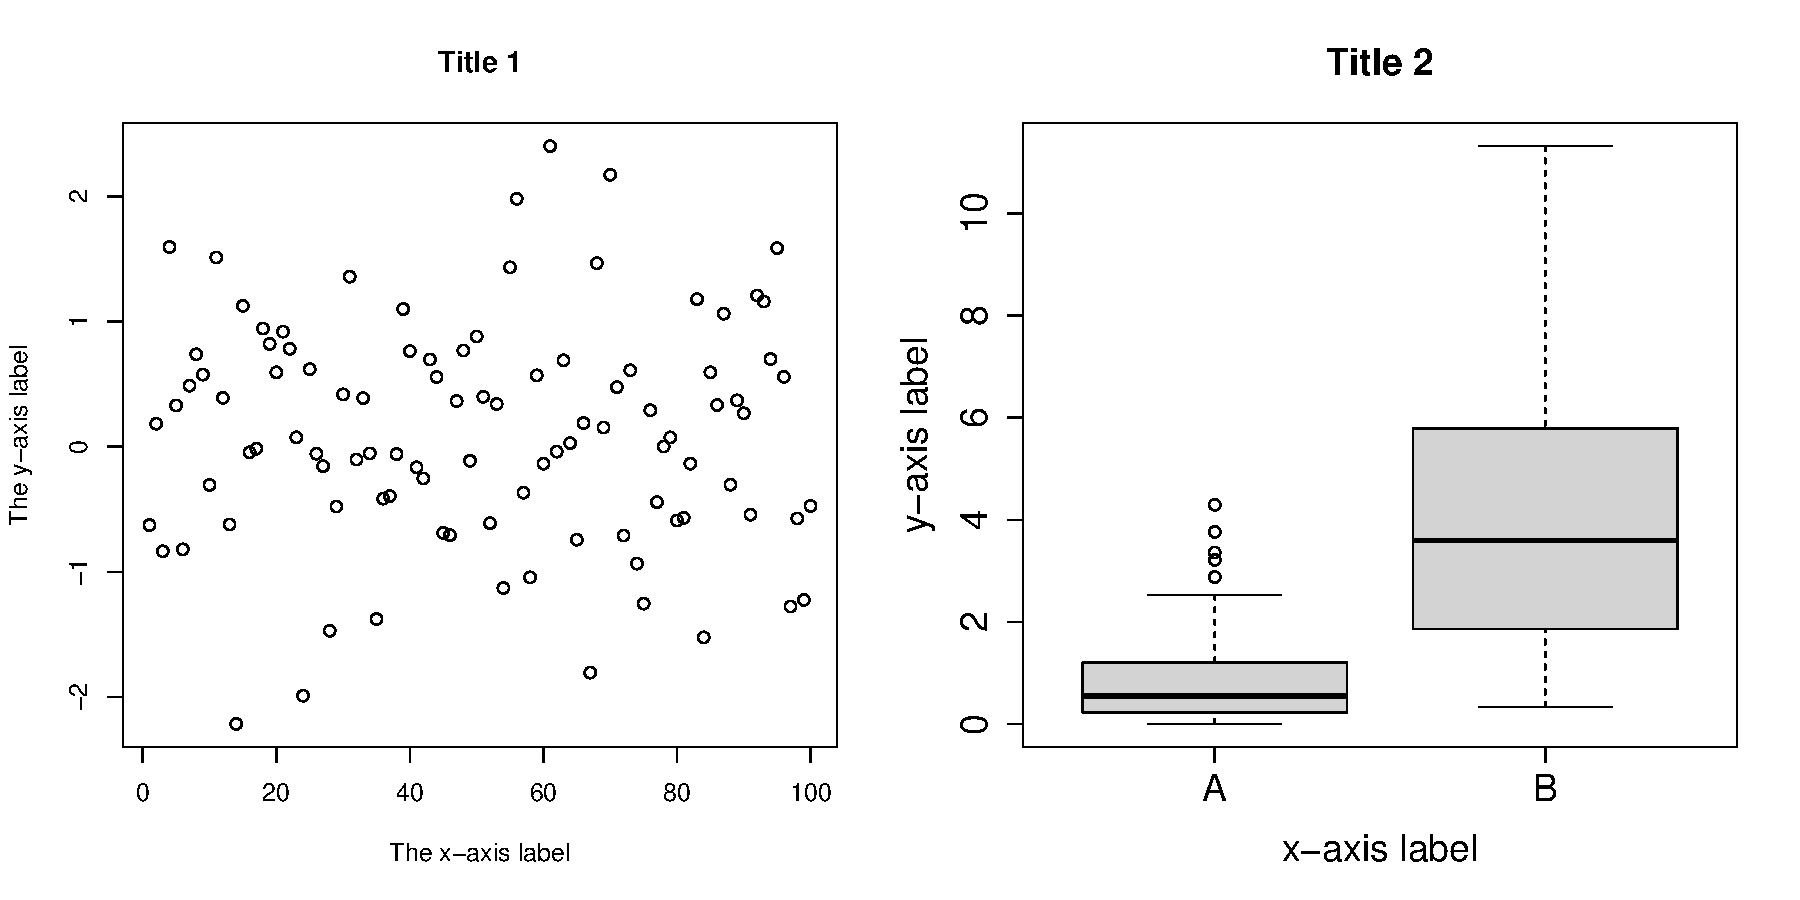
\includegraphics[width=0.9\textwidth]{images/fig1.pdf}
    \caption{An example scatterplot (left) and box plot (right).}
    \label{fig:axis-label-example}
\end{figure}

\section{Tables}\label{sec:tablesection}

\paragraph{Tips for the Tables.} Tables can be a useful way of displaying summary statistics. An example of a simple table is presented as Table~\ref{tab:normal}. All tables must be referenced in the main text of the report, in the order that they are referenced.

\begin{table}[ht]
\centering
\begin{tabular}{rr}
  \hline
    $z$& $\textrm{P}(Z < z)$ \\
  \hline
    1.281& 0.900\\
    1.645& 0.950\\
    1.960& 0.975\\
    2.326& 0.990 \\
    2.576& 0.995 \\
   \hline
\end{tabular}
    \caption{Partial table showing values of $z$ for $\textrm{P}(Z < z)$, 
    where $Z$ has a standard normal distribution.}
    \label{tab:normal}
\end{table}



\section{Referencing sources, sections and items} \label{sec:referencing}

\subsection{Referencing external sources}


Note that to make the references appear, you will need to compile the bibtex, otherwise you may just see question marks where the references should be. The small selection of example bibtex references used in this template are provided in the file \texttt{refs.bib}. These should be replaced with your own bibtex entries.
 
\subsection{Referencing elements of your report}

You might also want to cross reference results or claims from another part of your report such a as a section, result or equation. This is done by assigning a \texttt{\textbackslash label\{\}} to the item you wish to cross-reference and then using that label within \texttt{\textbackslash ref\{\}}. For example, Theorem~\ref{thm:variance-mse-relation} is proved in Section~\ref{sec:defnthms}. When referencing displayed mathematics, use \texttt{\textbackslash eqref\{\}}. As an example, see 
Equation~\eqref{eqn:variance-mse-relation}.

\subsubsection{Labelling tables and figures}

It is important that the label command
\texttt{\textbackslash label\{LABELNAME\}} comes \textbf{after} the caption command.
See Table~\ref{tab:normal} and Figure~\ref{fig:axis-label-example} as examples of this.

\subsection{Quoting sources}
If you wish to quote a source, be sure to use quotation marks and cite the
reference. The \texttt{\textbackslash{usequote}} command is useful here:


\section{Definitions, theorems and examples}
\label{sec:defnthms}

The following environments are supported:
Definition, Theorem, Proof, Proposition, Lemma, Remark, Example.

\begin{definition} \label{defn:variance}
    The \textbf{variance} of a random variable $X$ is defined as
    \begin{equation} \label{eqn:variance-definition}
        \mathrm{Var}(X) = \mathrm{E}[(X - \mathrm{E}[X])^2].
    \end{equation}
\end{definition}

\begin{theorem} \label{thm:variance-mse-relation}
Given a random variable $X$, over all values $a \in \mathbb{R}$, 
\begin{equation}
    \min_{a \in \mathbb{R}} \mathrm{E}[(X - a)^2] 
    = \mathrm{E}[(X - \mathrm{E}[X])^2].
    \label{eqn:variance-mse-relation}
\end{equation}
\end{theorem}

\begin{proof}   
    Starting with the left-hand side of Equation~\eqref{eqn:variance-mse-relation},
\begin{align}
% Example of using \newcommands; see above
\EE{ \inparenth{\X - \consta}^2 } 
&=  \EE{  \inparenth{\X - \EE{\X} + \EE{\X} - \consta}^2 } 
    \nonumber \\
&=  \EE{  \inparenth{ \X - \EE{\X} }^2 } 
    + 2 \EE{ \inparenth{ \X - \EE{\X} } \inparenth{ \EE{\X} - \consta} } +  
  \EE{ \inparenth{ \EE{\X} - \consta}^2  }    
    \nonumber \\
&=  \EE{  \inparenth{ \X - \EE{\X} }^2 } +  \inparenth{ \EE{\X} - \consta}^2
    \nonumber \\
& \geq \EE{  \inparenth{ \X - \EE{\X} }^2 },  
\nonumber 
\end{align}
since $\EE{\X}$ is a real number and $\inparenth{ \EE{\X} - \consta}^2 \geq 0$,
and the third line follows from linearity of expectation:
%
\begin{align}
    \EE{ \inparenth{ \X - \EE{\X} } \inparenth{ \EE{\X} - \consta} }
    =
    \inparenth{ \EE{\X} - \consta} \EE{ \inparenth{ \X - \EE{\X} } }
    =
    \inparenth{ \EE{\X} - \consta}  \inparenth{\EE{ \X} - \EE{\X} } 
    =
    0,
    \nonumber
\end{align}
%
since $\EE{\EE{\X}} = \EE{\X}$, which proves the result.
\end{proof}

\begin{remark}
    This theorem shows that that the minimum of the quantity
    $\mathrm{E}[(X - a)^2]$ is equal to $\mathrm{Var}(X)$.
    In some sense, this makes the variance a natural measure of dispersion if 
    we are taking the metric to be the squared deviation of $X$.
\end{remark}


\begin{lemma}[Stein's Lemma]
    Let $X \sim \mathrm{N}(\mu, \sigma^2)$, and let $g$ be a differentiable 
    function satisfying $\mathrm{E}[|g'(X)|] < \infty$. Then
    \begin{equation}
        \mathrm{E}[g(X)(X-\mu)] = \sigma^2 \mathrm{E}[g'(X)].
        \nonumber
    \end{equation}
\end{lemma}

\begin{proposition}[Popoviciu's inequality]
    Suppose that the random variable $X$ is known to only take values in the 
    bounded range $[a, b]$. Then  
    \begin{align}
        \mathrm{Var}[X] \leq \dfrac{(b-a)^2}{4}.
        \nonumber
    \end{align}
\end{proposition}

\begin{example}
    Suppose $X \sim \mathrm{Bern} (p)$, for some $p \in [0,1]$. Then, 
    since $X \in \{0, 1\}$, $X$ is bounded between $0$ and $1$ and so
    $\mathrm{Var}[X] \leq \tfrac{1}{4}$.
\end{example}

Note that Equations~\eqref{eqn:variance-definition} and \eqref{eqn:variance-mse-relation} are numbered because they are referred to elsewhere in the main text. All other equations are unnumbered. 

Each of these environments may be labelled and referenced as with sections. For example, we might discuss Definition~\ref{defn:variance} or Theorem~\ref{thm:variance-mse-relation} in this paragraph. 

%=========================================================


\end{document}
